\section{A Model of the Growth--Profitability Frontier}\label{sec:model}

This section builds a model in which a firm spends part of its revenue on growth, so that faster revenue growth costs current free cash flow margin. The model gives an efficient frontier between growth and margin and a closed form for the best attainable Rule-of-$X$ score. It identifies three limits on that score: market saturation, the finite headroom of market share, and competitive replication. It shows that, under a stated verification hypothesis, a value-maximizing firm maximizes a Rule-of-$X$ score at every date, with a weight equal to the marginal value of a dollar of revenue, and it explains how that weight relates to the weights investors use to screen firms. We then extend the model to heterogeneous firms, which relates it to the cross-sectional evidence of Section~\ref{sec:empirics}, and map the effects of AI automation onto its parameters. Finally, we charge the full cost of running AI against the ceiling of the score, derive the frontier a firm can reach by a given horizon when transitions are risky and organizational capacity is limited, and restate the objective in terms of economic profit for industries other than software. Supporting results are collected in Sections~\ref{supp:theory} and~\ref{app:theory} of the Supplementary Appendix, and all proofs are in Section~\ref{app:proofs} of the Supplementary Appendix. Results that follow directly from the functional form of the growth technology are stated as lemmas and remarks, and the free-entry result is a special case of a standard model. The results we believe are new are the score budget (\autoref{prop:budget}), the firm's decision weight on growth and its relation to the screening weights of investors (\autoref{prop:dynamic} and \autoref{lem:valuation2}), a worked instance of the classical non-identification of firm frontiers from chosen points, with within-firm co-movement (Propositions~\ref{prop:industry} and \ref{prop:industry-full}), the accountability floor as a control standard under common-mode failure (\autoref{prop:amin}), and the attainable and expected frontiers (Propositions~\ref{prop:attainable} and \ref{prop:expected}). The script \texttt{code/verify\_theory.py} checks the closed forms, first-order conditions and envelope derivatives symbolically, checks the concavity, limit, inequality and probability claims numerically on random parameter draws or by simulation, and labels as arithmetic the checks that verify only the numbers of an example.

\subsection{Setup}\label{sec:model-setup}

We describe a firm at a point in time. Revenue is $S$, the addressable market is $M$, and market share is $s=S/M$. Growth rates are instantaneous (continuously compounded) rates, so revenue growth equals market growth plus share growth. The two conventions for growth rates differ materially only at growth rates of the order of 100\% or more; Section~\ref{supp:model-rates} of the Supplementary Appendix states which results use which. Margins and spending are expressed as fractions of current revenue.

\begin{assumption}[Market and share]\label{ass:market}
The market grows at a constant nominal rate $G$. The firm's share satisfies $s\in(0,\bar s)$, where the cap $\bar s\in(0,1)$ reflects customer heterogeneity and, for share bought by acquisition, merger control. Revenue growth $g$ and share growth are linked by $g=G+\dot s/s$.
\end{assumption}

\begin{assumption}[Growth technology]\label{ass:growth}
The firm chooses discretionary growth spend $\sigma\in[0,\bar\sigma]$ (sales and marketing plus expansion R\&D, as a fraction of revenue). Here $\bar\sigma\in(0,\infty]$ is a financing cap, and $\bar\sigma=\infty$ means that spend can be financed externally without limit. Revenue grows at
\begin{equation}\label{eq:growth}
g \;=\; G+\lambda\,\sigma^{\alpha}\,h(s),\qquad h(s)=1-\frac{s}{\bar s},\qquad \alpha\in(0,1),\ \lambda>0 .
\end{equation}
We write $\ell:=\lambda h(s)>0$ for the firm's effective growth opportunity and $\Delta:=g-G\ge 0$ for excess growth.
\end{assumption}

The parameter $\lambda$ measures demand pull (the growth that spend buys when the share is small), $h(s)$ measures remaining headroom, and $\alpha<1$ imposes diminishing returns to spend. The technology resembles the sales-response model of \citet{vidale1957operations}, in which spend converts the unsaturated part of the market, and the goodwill model of \citet{nerlove1962optimal}; under a constant spend rate it makes the share follow a logistic path. It is a reduced form of models of customer capital and market penetration, which we take as given rather than derive: a rising marginal cost of reaching additional consumers \citep{arkolakis2010market} is what $\alpha<1$ and $h(s)$ stand for; spending on marketing and selling builds a customer base that is a slow-moving state variable \citep{gourio2014customer,drozd2012understanding}; and plant-level evidence shows that the accumulation of demand is driven mostly by plants' own past production decisions rather than by passive demand accumulation \citep{foster2016slow}. Two features of \eqref{eq:growth} are assumptions that matter later. Zero spend delivers market growth $G$, so no share is lost without spend (\autoref{rem:assumptions}(b) relaxes this). And growth cannot be traded below $G$ for margin: retention spending on customer success and support sits in the non-discretionary cost $a$ of \autoref{ass:costs}, and cutting it is not modeled as lowering growth.

\begin{assumption}[Costs]\label{ass:costs}
Gross margin is $\gamma=1-c_v$. Variable cost is $c_v=c_h+c_c+f$, made up of human service cost $c_h\ge 0$, compute (inference) cost $c_c\ge 0$ and third-party fees $f\ge 0$ (payments, marketplaces). Non-discretionary operating cost $a$ covers general and administrative cost, maintenance R\&D, and an accountability floor, and satisfies $a\ge a_{\min}\ge 0$. The operating margin is $m_{op}=\gamma-a-\sigma$, and $m_0:=\gamma-a$ is the margin intercept.
\end{assumption}

The margin intercept $m_0$ is an operating margin before growth spend. The free cash flow margin of a firm that grows with its market is lower by the capital that growth requires, $m_0-kG$ (\autoref{prop:frontier}(b)); where the distinction matters we call $m_0-kG$ the margin at market growth.

\begin{assumption}[Capital]\label{ass:capital}
Serving revenue requires a capital stock $K=kS$ with $k\ge 0$ (for example, owned compute), installed before the revenue it serves. Growth capital does not depreciate, and maintenance capital expenditure is included in $a$. The free cash flow (FCF) margin is
\begin{equation}\label{eq:fcf}
m \;=\; m_{op}-k\,g \;=\; m_0-\sigma-k\,g .
\end{equation}
\end{assumption}

Equation \eqref{eq:fcf} is exact in continuous time, because investment is $\dot K=k\dot S=kgS$, and in discrete time when capital is installed one period ahead; \autoref{lem:timing} in the Supplementary Appendix shows that the alternative, contemporaneous convention makes the feasible set non-convex for every $k>0$ when $\alpha<1/2$, and also for $\alpha\ge1/2$ when $k$ is large relative to $\kappa$ (defined below); for asset-light firms the non-convex region is a sliver just above market growth. Reported scores pair growth over the past year, $g_t$, with $\text{FCF}_t$, which is the contemporaneous convention; for firms whose capital expenditure leads revenue, $g_{t+1}+m_t$ is the pairing consistent with \eqref{eq:fcf}. Throughout, ``margin'' means the FCF margin $m$ unless stated otherwise. \autoref{rem:assumptions} in the Supplementary Appendix discusses fixed costs, firm-specific zero-spend growth, negative capital intensity, depreciation and network effects.

\begin{definition}[Feasible set, dominance, frontier, score]\label{def:frontier}
Fix $s$. The feasible set $\mathcal F$ is the set of pairs $(g,m)$ such that, for some $\sigma\in[0,\bar\sigma]$, $g=G+\ell\sigma^{\alpha}$ and $m\le m_0-\sigma-kg$ (margin can always be wasted). A pair $(g',m')$ dominates $(g,m)$ if $g'\ge g$ and $m'\ge m$, with at least one inequality strict. The efficient frontier is the set of undominated points of $\mathcal F$. For a weight $X\ge 0$, the Rule-of-$X$ score is $R_X(g,m)=Xg+m$. The Rule of 40 is the test $R_1\ge 0.40$, and Bessemer's Rule of $X$ uses weights $X$ of about 2 to 3.
\end{definition}

Table~\ref{tab:notation} in the Supplementary Appendix collects the notation of the paper. Four derived constants are used throughout:
\begin{equation}\label{eq:constants}
\beta:=\frac1\alpha>1,\qquad \kappa:=\ell^{-\beta}=(\lambda h)^{-\beta},\qquad y:=X-k,\qquad C_\alpha:=(1-\alpha)\,\alpha^{\alpha/(1-\alpha)}\in(0,1).
\end{equation}
The quantity $y$ is the net value of a unit of growth in the score: the weight $X$ less the capital $k$ that each unit of growth requires.


\paragraph{The spend elasticity $\alpha$.} The data do not identify the spend elasticity $\alpha$ (Section~\ref{sec:empirics}): under optimization spend and excess growth move in proportion (\autoref{prop:score}), so a log-log regression of one on the other has slope one whatever $\alpha$ is, and the ratio of growth spend to excess growth identifies only the product $\alpha(X-k)$. Elasticities from the marketing-response literature measure the response of the level of sales to advertising \citep{sethuraman2011advertising}, not that of excess growth to the spend share, so they do not map onto $\alpha$ either. We therefore treat $\alpha\in[0.25,0.45]$, equivalently $\beta=1/\alpha\in[2.2,4]$, as a scenario range, report sensitivity to it, and use $\alpha=0.3$ in every illustrative example. Two features of this range recur. First, since $\alpha<1/2$, the curvature of the frontier vanishes at $g=G$ (\autoref{prop:frontier}(c)): with $k\approx 0$ the frontier is nearly flat for modest excess growth and steepens sharply as $\Delta$ approaches $\ell$, the excess growth bought by spending 100\% of revenue. Second, for $\alpha<1/2$ the contemporaneous timing convention for growth capital makes the feasible set non-convex for every $k>0$; for $\alpha\ge1/2$ it does so only when $k$ is large relative to $\kappa$ (\autoref{lem:timing}).

\subsection{The efficient frontier}\label{sec:model-frontier}

\begin{lemma}[Efficient frontier]\label{prop:frontier}
Under Assumptions~\ref{ass:market}--\ref{ass:capital}, fix $s$ and let $\bar g:=G+\ell\bar\sigma^{\alpha}$ (with $\bar g=\infty$ if $\bar\sigma=\infty$). Write $I:=[G,\bar g]\cap\mathbb R$.
\begin{enumerate}
\item[(a)] The efficient frontier is the graph of
\begin{equation}\label{eq:frontier}
m^*(g)\;=\;m_0-k\,g-\kappa\,(g-G)^{\beta},\qquad g\in I .
\end{equation}
The feasible set $\mathcal F=\{(g,m):g\in I,\ m\le m^*(g)\}$ is convex. A feasible point is dominated if and only if $m<m^*(g)$. Each frontier point is produced by the unique spend level $\sigma=\kappa(g-G)^{\beta}$.
\item[(b)] At $g=G$ the frontier takes the value $m^*(G)=m_0-kG$, and its right derivative there is $-k$.
\item[(c)] $m^*$ is strictly decreasing and strictly concave on $I$. For $g>G$, $m^{*\prime}(g)=-k-\beta\kappa(g-G)^{\beta-1}$ and $m^{*\prime\prime}(g)=-\beta(\beta-1)\kappa(g-G)^{\beta-2}<0$. As $g\downarrow G$, $m^{*\prime\prime}(g)$ tends to $0$ if $\alpha<1/2$, equals $-2\kappa$ if $\alpha=1/2$, and tends to $-\infty$ if $\alpha>1/2$.
\item[(d)] If $\bar\sigma=\infty$, then as $g\to\infty$, $m^*(g)\to-\infty$, $m^{*\prime}(g)\to-\infty$ and $m^*(g)/g\to-\infty$.
\end{enumerate}
\end{lemma}

\noindent\emph{Intuition.} Growth is bought with spend, and because returns to spend diminish, each extra point of growth costs more margin than the one before. The frontier therefore bends down. Its slope at the market growth rate is only $-k$: the first unit of excess growth costs almost no spend, only the capital needed to serve it. The rate of steepening is governed by $\beta=1/\alpha$. Points strictly below the frontier waste margin.

\begin{figure}[t]
\centering
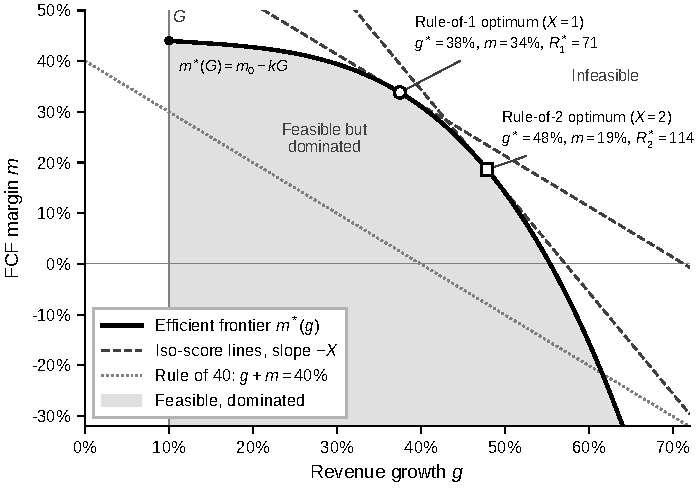
\includegraphics[width=0.64\linewidth]{figures/fig_frontier_tangency.pdf}
\caption{The efficient frontier and the Rule of $X$. The solid curve is the frontier $m^*(g)$ of \autoref{prop:frontier} for $m_0=0.45$, $G=0.10$, $k=0.10$, $\alpha=0.3$ and $\ell=0.6$; the shaded area is the set of feasible but dominated points. The dotted line is the Rule-of-40 boundary $g+m=0.40$. The dashed lines are iso-score lines of slope $-1$ and $-2$, tangent to the frontier at the Rule-of-1 and Rule-of-2 optima (markers) characterized in \autoref{prop:score}.}\label{fig:frontier}
\end{figure}

\subsection{The Rule of \texorpdfstring{$X$}{X} as a supporting line}\label{sec:model-score}

Geometrically, the frontier is a transformation curve between growth and margin, and a Rule-of-$X$ score is a price line with slope $-X$; its level sets are iso-score lines, not iso-value lines (\autoref{prop:general}(c)). The tangency between the two has antecedents in the growth-valuation frontier of the managerial firm \citep{marris1964economic,solow1971some,odagiri1981theory}, and recent firm-level evidence that firms grow by acquiring customers through marketing and distribution at roughly constant markups supports the growth technology behind it \citep{fitzgerald2024how,argente2025how,afrouzi2023concentration}. Given the functional form, the closed forms below are a routine power-function calculation.

\begin{lemma}[Maximal Rule-of-$X$ score]\label{prop:score}\label{prop:optimum}
Fix $X\ge 0$ and $s$. In parts (b) and (e), assume that the financing cap does not bind, that is, $\sigma^*\le\bar\sigma$ with $\sigma^*$ given in \eqref{eq:sigstar}; this always holds if $\bar\sigma=\infty$.
\begin{enumerate}
\item[(a)] Iso-score sets $\{(g,m):Xg+m=c\}$ are straight lines of slope $-X$. A maximizer of $R_X$ on $\mathcal F$ exists, and every maximizer lies on the frontier.
\item[(b)] If $X>k$, the maximizer is unique and interior ($g^*>G$), and there the frontier is tangent to the iso-score line: $m^{*\prime}(g^*)=-X$ (if $\sigma^*=\bar\sigma$, the maximizer is the right endpoint $\bar g$ of $I$ and the tangency holds for the left derivative). In closed form,
\begin{align}
\Delta^* &= g^*-G=(\lambda h)^{1/(1-\alpha)}\,\bigl[\alpha(X-k)\bigr]^{\alpha/(1-\alpha)}, \label{eq:Dstar}\\
\sigma^* &= \bigl[\alpha\lambda h\,(X-k)\bigr]^{1/(1-\alpha)} \;=\; \alpha(X-k)\,\Delta^*, \label{eq:sigstar}\\
R_X^* &= m_0+(X-k)\,G+(1-\alpha)(X-k)\,\Delta^* \;=\; m_0+(X-k)\,G+C_\alpha\bigl[\lambda h\,(X-k)\bigr]^{1/(1-\alpha)}, \label{eq:Rstar}
\end{align}
and the margin at the optimum is $m^*(g^*)=m_0-kg^*-\alpha(X-k)\Delta^*$.
\item[(c)] If $X\le k$, the unique maximizer is the corner $g^*=G$ with $\sigma^*=0$, and $R_X^*=m_0+(X-k)G$. This part does not need the cap condition.
\item[(d)] (Duality.) Each frontier point with $G<g<\bar g$ is the unique maximizer of $R_X$ for exactly one weight, $X(g)=-m^{*\prime}(g)=k+\beta\kappa(g-G)^{\beta-1}$. The point $g=G$ is a maximizer if and only if $X\le k$. If $\bar\sigma=\infty$, the optimal growth rate $g^*(X)$ is continuous and nondecreasing in $X$, and strictly increasing for $X>k$.
\item[(e)] The growth surplus $\Pi:=(1-\alpha)(X-k)\Delta^*$ (zero if $X\le k$) satisfies $\Pi=\max_{\sigma\ge 0}\{(X-k)\,\ell\,\sigma^{\alpha}-\sigma\}$, so that $R_X^*=m_0+(X-k)G+\Pi$.
\end{enumerate}
\end{lemma}

When the dependence matters we write $\Delta^*(\ell,X)$ and $\sigma^*(\ell,X)$ for \eqref{eq:Dstar} and \eqref{eq:sigstar} with $\lambda h$ replaced by $\ell$ and $X-k$ by $(X-k)_+$.

\noindent\emph{Intuition.} Because the feasible set is convex, maximizing a linear score is a supporting-line problem: push a line of slope $-X$ outward until it last touches the frontier. The maximal score has three parts. The intercept $m_0$ is what the firm earns without outgrowing its market. The term $(X-k)G$ is the value of the free growth the market supplies, net of the capital it requires. The growth surplus $\Pi$ is the profit from running the growth technology at a shadow price of $X-k$ per unit of growth. The spend rule $\sigma^*=\alpha(X-k)\Delta^*$ is a \citet{dorfman1954optimal} condition: spend equals the spend elasticity times the value of the growth it buys, so the fraction $\alpha$ of that value is spent and the fraction $1-\alpha$ is kept as surplus. When the weight on growth does not cover the capital each unit of growth needs ($X\le k$), the firm should buy no growth. Part (d) says the weight $X$ indexes the frontier: choosing a rule is the same as choosing a point.

Remarks~\ref{rem:cap} and \ref{rem:r40} in the Supplementary Appendix treat a binding financing cap and show that the Rule of 40, read as a pass mark, accepts an interval of frontier points and dominated points below them, whereas the Rule of $X$ selects one. \autoref{rem:general-phi} separates the results that hold for any increasing concave growth technology from those specific to the isoelastic form \eqref{eq:growth}.

\subsection{Limits: saturation, small base and the score budget}\label{sec:model-limits}

Write $R_X^*(s)$ for the maximal score at share $s$ when $\bar\sigma=\infty$, let $y_+:=\max\{X-k,0\}$, and define the saturated score
\begin{equation}\label{eq:Rinf}
R_\infty:=m_0+(X-k)\,G .
\end{equation}

\begin{lemma}[Saturation and the small-base bound]\label{prop:saturation}
Fix $X\ge 0$ and let $\bar\sigma=\infty$.
\begin{enumerate}
\item[(a)] $R_X^*(s)=R_\infty+C_\alpha\bigl[\lambda h(s)\,y_+\bigr]^{1/(1-\alpha)}$. If $X>k$, this is strictly decreasing in $s$, with $dR_X^*/ds=-(X-k)\Delta^*/(\bar s-s)$. If $X\le k$, it is constant.
\item[(b)] (Saturation limit.) $\lim_{s\to\bar s}R_X^*(s)=R_\infty$. For the Rule of 40 with $k=0$, the limit is $m_0+G$. Since $m_0=1-c_h-c_c-f-a\le 1-c_c-f-a_{\min}\le 1$,
\begin{equation}\label{eq:rule100}
R_\infty\;\le\;1-c_c-f-a_{\min}+(X-k)\,G,\qquad\text{and for }X=1:\quad R_\infty\le 1+(1-k)\,G .
\end{equation}
\item[(c)] (Small-base bound.) $\sup_{s\in(0,\bar s)}R_X^*(s)=\lim_{s\to 0}R_X^*(s)=R^0:=R_\infty+C_\alpha(\lambda y_+)^{1/(1-\alpha)}$. If $X>k$, the supremum is not attained; if $X\le k$, $R_X^*$ is constant in $s$ and the supremum is attained at every share.
\item[(d)] (Demand-pull threshold.) Let $X>k$ and $\bar R>R_\infty$, and define
\begin{equation}\label{eq:Lambda}
\Lambda(\bar R):=\frac{1}{X-k}\left[\frac{\bar R-R_\infty}{C_\alpha}\right]^{1-\alpha}.
\end{equation}
Then $R_X^*(s)\ge\bar R$ if and only if $\lambda h(s)\ge\Lambda(\bar R)$, and a score of $\bar R$ is attainable at some share if and only if $\lambda>\Lambda(\bar R)$. A firm exactly at the threshold has $\Delta^*=(\bar R-R_\infty)/[(1-\alpha)(X-k)]$, $\sigma^*=\alpha(\bar R-R_\infty)/(1-\alpha)$ and $m=m_0-kg^*-\sigma^*$.
\end{enumerate}
\end{lemma}

\noindent\emph{Intuition.} Rising share uses up growth opportunity. As $s\to\bar s$, the growth surplus vanishes and the best score falls to the margin intercept plus the value of free market growth. Because the margin intercept cannot exceed 100\% of revenue, a saturated firm with negligible capital cannot sustain a Rule-of-40 score above $100(1+G)$ points. With $G$ between 0.05 and 0.30, this is the formal content of a ``Rule of about 100''. Scores far above that level need demand pull above the threshold \eqref{eq:Lambda}, and even then only at small share, with very large spend and deeply negative margins. With $\alpha=0.3$, $X=1$, $k=0$, $m_0=0.6$ and $G=0.2$ ($R_\infty=0.8$), a ``Rule of 1000'' requires $\lambda h\ge\Lambda\approx 8.71$; at the threshold the firm grows about 1{,}314 points faster than its market, spends about 394\% of revenue on growth and runs an FCF margin of about $-334\%$, in continuously compounded rates. \autoref{prop:myopic} in the Supplementary Appendix adds that, if the firm spends at the static optimum for a fixed weight at every date (a myopic policy, not the dynamically optimal one of \autoref{prop:dynamic}), its excess over $R_\infty$ decays at least as fast as $t^{-1/\alpha}$.

\begin{figure}[t]
\centering
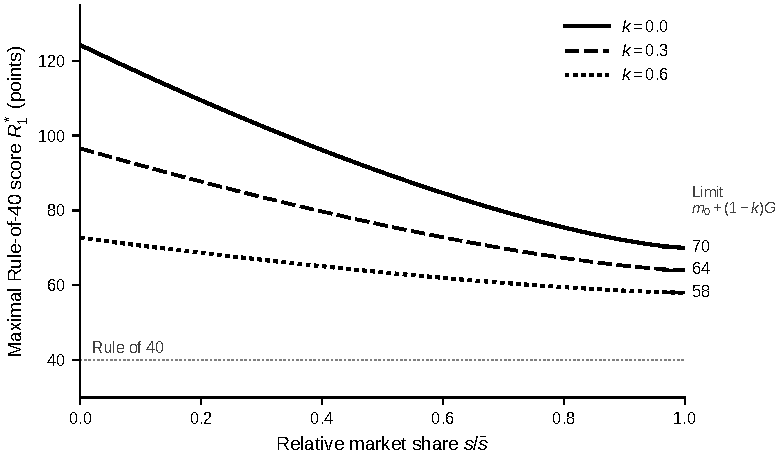
\includegraphics[width=0.64\linewidth]{figures/fig_saturation.pdf}
\caption{Saturation. The maximal Rule-of-40 score $R_1^*$ of \autoref{prop:saturation}(a) as a function of the relative share $s/\bar s$, for capital intensities $k\in\{0,0.3,0.6\}$, with $m_0=0.50$, $G=0.20$, $\lambda=1.2$ and $\alpha=0.3$. Each curve falls to its saturation limit $m_0+(1-k)G$, marked by a horizontal tick and label at the right edge. The dotted line marks a score of 40.}\label{fig:saturation}
\end{figure}

The next result makes the transience of extreme scores precise. It needs neither the functional form \eqref{eq:growth} nor optimal behavior. It needs the margin bound $m\le m_0-kg$, growth of at least $G$ at every spend level (no share is lost without spend), and share accounting in a single market whose size grows exogenously at $G$ under a fixed cap $\bar s$.

\begin{proposition}[Score budget]\label{prop:budget}
Let the firm sell in a single market whose size grows exogenously at rate $G$, with a fixed share cap $\bar s$, and let its growth be at least $G$ whatever its spend. Hold $m_0$, $G$, $k$ and $X>k$ fixed, and let $R_\infty=m_0+(X-k)G$.
\begin{enumerate}
\item[(a)] (Continuous time.) Take any measurable spend path $\sigma:[0,T]\to[0,\bar\sigma]$ with $\int_0^T\sigma^{\alpha}\,dt<\infty$, any measurable margins $m(t)\le m_0-\sigma(t)-k\,g(t)$, and the induced share path from $s(0)=s_0$. Then
\begin{equation}\label{eq:budget}
\int_0^T\bigl(R_X(t)-R_\infty\bigr)^+\,dt\;\le\;(X-k)\,\ln\frac{s(T)}{s_0}\;<\;(X-k)\,\ln\frac{\bar s}{s_0}.
\end{equation}
\item[(b)] (Discrete time.) Suppose instead that growth and margins are period rates, with $G>-1$: $s_{t+1}=s_t(1+g_t)/(1+G)$, $g_t\ge G$, $m_t\le m_0-kg_t$, and $s_t\le\bar s$ for all $t$. Then
\begin{equation}\label{eq:budget-discrete}
\sum_{t=0}^{T-1}\ln\!\Bigl(1+\frac{(R_{X,t}-R_\infty)^+}{(X-k)(1+G)}\Bigr)\;\le\;\ln\frac{s_T}{s_0}\;\le\;\ln\frac{\bar s}{s_0}.
\end{equation}
\item[(c)] (Moving intercept.) If the margin intercept moves over time, $m_0(t)$, then (a) and (b) hold with $R_\infty(t)=m_0(t)+(X-k)G$ in place of $R_\infty$.
\end{enumerate}
\end{proposition}

\noindent\emph{Intuition.} Every point of score above the saturated level must be paid for with excess growth, and excess growth is share growth. Share can grow only from $s_0$ to $\bar s$, so the log headroom $\ln(\bar s/s_0)$ is a finite budget that every growth strategy draws on. A firm can spend the budget quickly, on a high but brief score, or slowly, on a modest but long-lived one; \autoref{prop:budget-sharp} in the Supplementary Appendix shows that the bound \eqref{eq:budget} is sharp, and is approached only by slow spending: a firm that spends fast converts headroom into score at a lower rate, because spend rises more than proportionally with excess growth (\autoref{cor:transient}(b)). Within one market, and with zero-spend growth at least equal to market growth, a firm cannot spend the budget twice. The budget is finite only under those conditions: a firm whose retention lags its market loses share without spending and can buy it back repeatedly (\autoref{rem:assumptions}(b)), a firm that acquires businesses in markets it does not yet serve buys new headroom with each deal (\autoref{prop:acquired-score}(e)), and a firm that creates a new market with a new product opens a new budget in that market. The proposition bounds score per market at given retention, not the score of a firm that keeps entering markets.

\begin{corollary}[Extreme scores are transient]\label{cor:transient}
Let $X>k$ and $\bar R>R_\infty$.
\begin{enumerate}
\item[(a)] (Period rates.) In the setting of \autoref{prop:budget}(b), the number $\mathcal T(\bar R)$ of periods in which a firm starting at share $s_0$ scores at least $\bar R$ satisfies
\begin{equation}\label{eq:transient}
\mathcal T(\bar R)\;\le\;\frac{\ln(\bar s/s_0)}{\ln\bigl(1+(\bar R-R_\infty)/[(X-k)(1+G)]\bigr)} .
\end{equation}
\item[(b)] (Continuous time.) In the setting of \autoref{prop:budget}(a), the time a firm spends at or above $\bar R$ is at most $(X-k)\ln(\bar s/s_0)/(\bar R-R_\infty)$. Under the growth technology \eqref{eq:growth}, a firm that sets spend at the static optimum for the weight $X$ at every date (\autoref{prop:myopic}) spends at most $(1-\alpha)(X-k)\ln(\bar s/s_0)/(\bar R-R_\infty)$ there.
\end{enumerate}
For example, let $X=1$, $k=0$, $m_0=0.6$ and $G=0.2$ (so $R_\infty=0.8$), with $\bar s=0.5$. In annual periods, from $s_0=1\%$ the firm can score at least 1{,}000 points ($R_1\ge 10$) in at most one year (the bound is 1.8) and at least 140 points in at most nine years (bound 9.6); from $s_0=10^{-5}$ it can score at least 1{,}000 points in at most five years (bound 5.0). In continuous time, from $s_0=1\%$ it can score at least 1{,}000 points for at most 0.43 years, and for at most 0.30 years at the static optimum.
\end{corollary}

\subsection{Comparative statics}\label{sec:model-statics}

\begin{lemma}[Envelope results]\label{prop:envelope}\label{prop:capital}
Let $\bar\sigma=\infty$ and $X\ge 0$. The maximal score $R_X^*$ is continuously differentiable in $(m_0,G,k,X,\lambda,s)$, with
\begin{equation}\label{eq:envelope}
\begin{gathered}
\frac{\partial R_X^*}{\partial m_0}=1,\qquad
\frac{\partial R_X^*}{\partial G}=X-k,\qquad
\frac{\partial R_X^*}{\partial k}=-g^*,\qquad
\frac{\partial R_X^*}{\partial X}=g^*,\\
\frac{\partial R_X^*}{\partial\lambda}=\frac{(X-k)\Delta^*}{\lambda}=(X-k)\,h\,(\sigma^*)^{\alpha}\ge 0,
\end{gathered}
\end{equation}
where the last inequality is strict if and only if $X>k$. Through $m_0=\gamma-a$ and $\gamma=1-c_h-c_c-f$, $\partial R_X^*/\partial\gamma=1$ and $\partial R_X^*/\partial a=\partial R_X^*/\partial c_c=-1$. Moreover $R_X^*$ is convex in $k$ and in $\lambda$, and $\partial^2R_X^*/\partial k\,\partial\lambda=-\Delta^*/[(1-\alpha)\lambda]\le 0$.
\end{lemma}

\noindent\emph{Intuition.} By the envelope theorem, a parameter change can be valued at the optimal point without re-optimizing. Capital intensity is charged on every unit of growth, including the free market growth, so its marginal cost is the growth rate itself. The negative cross-partial says that firms with more growth opportunity are hurt more by capital intensity.

\begin{corollary}[Capital-for-labor substitution]\label{cor:capital}\label{cor:substitution}
Let $\bar\sigma=\infty$, and suppose automation lowers $a$ by $da>0$ and raises $k$ by $dk>0$, with other parameters fixed. Then the change in the maximal score satisfies
\begin{equation}\label{eq:kl-bracket}
da-g^*(k)\,dk\;\le\;\Delta R_X^*\;\le\;da-g^*(k+dk)\,dk .
\end{equation}
Hence the score rises if $da>g^*(k)\,dk$ and does not rise if $da\le g^*(k+dk)\,dk$. To first order, it rises if and only if $da>g^*\,dk$.
\end{corollary}

\noindent\emph{Intuition.} Replacing recurring human cost with owned capital raises the FCF score only if the opex saved per dollar of revenue exceeds the growth rate times the added capital per dollar of revenue, because the capital must be bought again for every new dollar of revenue. Without depreciation, raising $k$ by 0.10 must cut opex by more than 5 points of revenue for a firm growing at 50\%, but by only 1 point for a firm growing at 10\%. Compute depreciates quickly, however: with depreciation at rate $\delta_K$ the threshold becomes $(g^*+\delta_K)\,dk$ (\autoref{rem:assumptions}(c)), so at $\delta_K=0.25$ the two figures rise to 7.5 and 3.5 points. The bracket \eqref{eq:kl-bracket} holds exactly, not only to first order, because $R_X^*$ is convex in $k$.

\begin{corollary}[Automation priorities]\label{cor:priorities}
Let $\bar\sigma=\infty$ and $X>k$, so that the Rule-of-$X$ optimum is interior, and evaluate each improvement at the optimum, with spend re-optimized and the weight $X$ held fixed. To first order:
\begin{enumerate}
\item[(i)] (Non-discretionary cost.) Removing non-discretionary cost $da$ (a share of revenue) raises $R_X^*$ by $da$ and the saturated score $R_\infty$ by $da$, so the gain survives saturation.
\item[(ii)] (Growth engine.) Let an improvement $x$ in the efficiency of growth spend deliver the same growth for spend $\sigma/(1+x)$, which maps to $\lambda\mapsto\lambda(1+x)^{\alpha}$. It raises $R_X^*$ by $x\,\sigma^*$, the same as cutting a non-discretionary cost line of size $\sigma^*$ by the proportion $x$; exactly, by $\Pi[(1+x)^{\alpha/(1-\alpha)}-1]$. Measured instead as a rise $x_\lambda$ in demand pull, the gain is $x_\lambda(X-k)\Delta^*=x_\lambda\,\sigma^*/\alpha$ to first order and $\Pi[(1+x_\lambda)^{1/(1-\alpha)}-1]$ exactly; the factor $1/\alpha$ between the two reflects only the unit in which the improvement is measured. Neither raises $R_\infty$, and both vanish as $s\to\bar s$.
\item[(iii)] (Retention.) Raising zero-spend growth $G_i$ (net revenue retention, \autoref{rem:assumptions}(b)) by $dG$ raises $R_X^*$ by $(X-k)\,dG$, and $R_\infty$ by the same amount; at a fixed weight the gain does not depend on the firm's share or growth.
\item[(iv)] (Cost of revenue.) A cut $du<0$ in unit cost of revenue raises the gross margin, and hence $R_X^*$, by $(1-\epsilon_p)|du|/p$ at given demand, where $\epsilon_p$ is the pass-through elasticity of \autoref{lem:prices}. Under free entry without a scarce input it leaves the long-run markup at zero (\autoref{prop:entry}(b)); the long-run score then changes only through the normal return on capital and customer capital, $(r-G)(k_u+a_c)/\hat c$, because lower prices raise capital per dollar of revenue, and not at all if $k_u+a_c=0$.
\item[(v)] (Capital for labor.) Automation that adds capital $dk$ while removing cost $da$ raises $R_X^*$ if and only if $da>g^*dk$ (\autoref{cor:capital}); since $g^*\ge G$, the hurdle is lowest for the slowest growers.
\end{enumerate}
\end{corollary}

\noindent\emph{Intuition.} At a fixed weight, the gain from cutting non-discretionary cost survives saturation (part (i)), the gain from a better growth engine vanishes with it (part (ii)), savings in cost of revenue count only to the extent the firm keeps them (part (iv)), and capital-heavy automation suits slow growers (part (v)). A ranking by stage needs one more step. If the firm acts on its own decision weight $X^{\mathrm{dyn}}(s)=v'(s)$ of \autoref{prop:dynamic}, which in the worked example there falls from \VpOnePct{} at 1\% of the cap to about \VpMin{} near \VpMinAt\% and stays below its small-share values up to saturation, then the gains in (ii) and (iii), both proportional to $X-k$, are larger for a firm at small share, although near saturation the retention gain of (iii) is still about \VpGainShare\% of its small-share value; at a common fixed weight, only the saturation of (ii) distinguishes stages. Parts (i) and (iii) treat cost and retention as independent levers, but spending on customer success and support sits in $a$ and sustains retention, so cutting it may lower $G_i$. These are effects that shift the frontier itself, distinct from closing a firm's distance to its frontier.

\subsection{Which weight on growth? The firm's and the investor's}\label{sec:model-valuation}

The score results take the weight $X$ as given. Which weight should a firm use, and how does it relate to the weights of 2 to 3 in investors' screens? We answer the first question with the firm's dynamic problem and the second with a valuation identity. Both weights turn out to be marginal rates of substitution between growth and margin in value; they price perturbations of different persistence. The dynamic problem belongs to the class of optimal-advertising problems with a saturating sales response \citep{sethi1973optimal,sethi1977dynamic,feichtinger1994dynamic}, in which the costate is the marginal value of sales, and the firm's weight is the counterpart of the shadow value of customer capital \citep{gourio2014customer} or brand capital \citep{vitorino2014understanding} in models of marketing as investment; in the investment model of \citet{belo2022decomposing}, brand capital accounts for 6\% to 25\% of firm value, depending on the industry. What we add is the reading of the optimum, under (H), as a Rule-of-$X$ score at every date and the comparison of that weight with the weights investors screen on.

Let $r>G$ be the discount rate. A spend policy is a measurable $\sigma:[0,\infty)\to[0,\infty)$ with $\int_0^t\sigma^{\alpha}d\tau<\infty$ for all $t$. Under Assumptions~\ref{ass:market}--\ref{ass:capital} it induces, from $s(0)=s_0$, the share path $\dot s=s\,\ell(s)\,\sigma^{\alpha}$ with $\ell(s)=\lambda h(s)$, revenue $S_t=s_tM_t$ and FCF margin $m_t=m_0-\sigma_t-kg_t$. Firm value is
\begin{equation}\label{eq:value}
V(S_0,M_0):=\sup_{\sigma}\ \limsup_{T\to\infty}\int_0^Te^{-rt}\,m_t\,S_t\,dt,
\end{equation}
where each integral is well defined in $[-\infty,\infty)$ because $m_t\le m_0-kG$.

\begin{proposition}[Dynamic optimality: under (H), the firm's own growth weight is the marginal $q$ of revenue]\label{prop:dynamic}
Let $\bar\sigma=\infty$, $r>G$ and $m_0-kG>0$.
\begin{enumerate}
\item[(a)] (Homogeneity.) $V(S,M)=M\,v(S/M)$, where $v(s):=V(s,1)$ satisfies $(m_0-kG)\,s/(r-G)\le v(s)\le(m_0-kG)\,\bar s/(r-G)$. Hence $\partial V/\partial S=v'(s)$, the marginal value of a dollar of revenue, and $V/S=v(s)/s$, the revenue multiple, wherever $v$ is differentiable.
\item[(b)] (Verification.) Let $\hat v\in C^1((0,\bar s))$ be bounded and satisfy the Hamilton--Jacobi--Bellman (HJB) equation
\begin{equation}\label{eq:hjb}
(r-G)\,\hat v(s)\;=\;s\max_{\sigma\ge 0}\bigl\{m_0-\sigma-kG+\bigl(\hat v'(s)-k\bigr)\,\ell(s)\,\sigma^{\alpha}\bigr\}\qquad\text{for all }s\in(0,\bar s).
\end{equation}
Then $\hat v\ge v$. Say that the verification hypothesis (H) holds if such a $\hat v$ exists and, from every $s_0\in(0,\bar s)$, the feedback $\hat\sigma(s)=\sigma^*(\ell(s),\hat v'(s))$ generates a share path in $(0,\bar s)$. Under (H), $\hat v=v$ and the feedback is optimal.
\item[(c)] (The Rule of $X$ at every date.) The maximand in \eqref{eq:hjb} equals $R_X(g,m)-XG$ with $X=\hat v'(s)$. Under (H), a firm that follows the optimal feedback therefore maximizes, at every date, the Rule-of-$X$ score at its current share, with weight
\begin{equation}\label{eq:Xdyn}
X^{\mathrm{dyn}}(s)\;=\;v'(s)\;=\;\frac{\partial V}{\partial S},
\end{equation}
the marginal $q$ of revenue; and \eqref{eq:hjb} can be written $R^*_{X^{\mathrm{dyn}}(s)}(s)=(r-G)\,v(s)/s+G\,X^{\mathrm{dyn}}(s)$.
\item[(d)] (Small share.) Let $v_0$ be the smallest positive number that satisfies
\begin{equation}\label{eq:gordon}
(r-G)\,v_0\;=\;m_0-kG+C_\alpha\bigl[\lambda\,(v_0-k)_+\bigr]^{1/(1-\alpha)},
\end{equation}
assumed to exist and to be a simple root, and let $\Delta^\circ=\Delta^*(\lambda,v_0)$, $\sigma^\circ=\sigma^*(\lambda,v_0)$, $g^\circ=G+\Delta^\circ$ and $m^\circ=m_0-kg^\circ-\sigma^\circ$. Then $g^\circ<r$ and $v_0=m^\circ/(r-g^\circ)$; $v(s)\le v_0\,s$ for all $s$; and $\lim_{s\to 0}v(s)/s=v_0$. Under (H), also $X^{\mathrm{dyn}}(s)=\hat v'(s)\to v_0$ as $s\to 0$.
\item[(e)] (No root.) If \eqref{eq:gordon} has no positive root, then $v(s)/s\to\infty$ as $s\to 0$.
\end{enumerate}
\end{proposition}

Parts (a), (d) and (e) hold unconditionally; parts (b) and (c) state what follows if (H) holds. We have not proved (H). It is the hypothesis of a verification theorem, and we state it as an assumption. Where spend is positive, \eqref{eq:hjb} is equivalent to an explicit first-order ordinary differential equation in $v$ that is singular at both ends of $(0,\bar s)$ (Section~\ref{app:proofs} of the Supplementary Appendix). For the parameters of the worked example below, a numerical solution of \eqref{eq:hjb} by dynamic programming on a fine grid has a smooth profile, and its feedback generates admissible paths (\texttt{code/verify\_theory.py}, checks 15g to 15m). That is evidence for (H) at those parameters, not a proof. Two consequences of \eqref{eq:hjb} show what (H) requires. If $(m_0-kG)/(r-G)\le k$, the linear function $\hat v(s)=(m_0-kG)s/(r-G)$ solves \eqref{eq:hjb}, so (H) holds and the firm never spends on growth. If $(m_0-kG)/(r-G)>k$, no solution has a region without spend, so under (H) the firm spends at every share, and $\hat v$ must meet the terminal condition $\hat v(\bar s)=(m_0-kG)\bar s/(r-G)$; the numerical solution passes through that singular point. The second condition of (H), that the feedback generates a share path, then holds automatically, so the content of (H) is the existence of a bounded continuously differentiable solution of \eqref{eq:hjb} on $(0,\bar s)$. Every statement in this paper that a value-maximizing firm acts on a weight equal to the marginal value of revenue is conditional on (H).

\noindent\emph{Intuition.} A point of excess growth bought today is a permanent addition to the revenue base, worth $v'(s)$ per dollar of revenue, while the spend that buys it is paid once. Under (H), the HJB equation splits the firm's problem into a sequence of static Rule-of-$X$ problems, one per date, with a weight equal to the marginal value of revenue. The Rule of $X$ is then the right instantaneous criterion, and its weight is a marginal value of revenue, not a fixed 2 or 3. \citet{hayashi1982tobin} shows that marginal and average $q$ coincide when value is linearly homogeneous in the stock. Here value is homogeneous of degree one in revenue and market size jointly, not in revenue alone, so saturation drives marginal $q$ of revenue, $v'(s)$, apart from the revenue multiple $v(s)/s$. The two coincide in the small-share limit of part (d), where the firm is a constant-growth firm whose revenue multiple $v_0=m^\circ/(r-g^\circ)$ is the Gordon multiple. Part (e) is the case in which the growth technology allows growth at a rate close to the discount rate with a positive margin, so that the small-share multiple is unbounded.

\noindent\emph{Worked example.} In the example of Section~\ref{supp:model-weights} of the Supplementary Appendix, under (H), a firm whose revenue multiple at a small share is 10 acts on a growth weight of \VpOnePct, \VpTenPct{} and \VpFiftyPct{} at 1\%, 10\% and 50\% of its share cap, close to and below its revenue multiple; the weight falls to about \VpMin{} near \VpMinAt\% of the cap and then rises toward the never-spend multiple of \VpLimit; a multiple of 15 gives correspondingly higher weights. In the example the weight lies below the revenue multiple at every share, so the firm's own weight exceeds the screening weights of 2 to 3 when its revenue multiple is well above three; at a higher discount rate both are lower.

\noindent\emph{Implication for measurement.} Because $\sigma^*=\alpha(X-k)\Delta^*$, the ratio of growth spend to excess growth over market growth reveals $\alpha(X-k)$, and since $\alpha<1$ it bounds the net weight from below whatever $\alpha$ is: $X-k=(\sigma^*/\Delta^*)/\alpha>\sigma^*/\Delta^*$. Conditional on $\alpha$, a spend ratio $\hat\rho$ implies $X-k=\hat\rho/\alpha$, between $2.2\hat\rho$ and $4\hat\rho$ for $\alpha\in[0.25,0.45]$. The data observe neither growth spend nor excess growth over market growth. The selling-and-marketing share also contains spending that maintains revenue, and excess growth is measured against the sample median rather than against $G$. Section~\ref{sec:empirics} reports the values of $\alpha(X-k)$ that different proxies give: from \AlphaAllLo{} to \AlphaAllHi{} across methods, so that $X-k$ ranges from about \XkLo{} to about \XkHi{} for $\alpha\in[0.25,0.45]$. The spend data therefore do not identify the decision weight. Under (H), whether a firm's decision weight exceeds the screening weights is therefore a statement about its revenue multiple (part (c) and the worked example), not a finding from spending data. Where an example below needs a weight, we evaluate it at $X\in\{2.5,5,9\}$ and say where its conclusion changes below 2.5.

The weights in investors' screens answer a different question. They compare a change in the growth rate that persists for several years with a change in the margin, which is what regressions of revenue multiples on growth and margin estimate. Let $\eta:=(1+g)/(1+r)$, $\mathcal N_T(\eta):=\sum_{t=1}^T\eta^t$, and let $\mathcal M_\infty:=(1+G_\infty)/(r-G_\infty)$ be a Gordon multiple for growth $G_\infty\in(-1,r)$ after year $T$.

\begin{lemma}[The investor's screening weight]\label{lem:valuation2}\label{lem:valuation}\label{lem:ruleX}
Let $V=S_0\,[\,m\,\mathcal N_T(\eta)+m_{LR}\,\eta^T\mathcal M_\infty\,]$: revenue grows at $g$ for $T$ years and at $G_\infty$ thereafter, the current margin $m$ holds for $T$ years, and the long-run margin is $m_{LR}=\theta m+(1-\theta)\bar m$, where $\theta\in[0,1]$ measures the persistence of the current margin and $\bar m$ is the margin the business earns at maturity. Define $X^{\mathrm{scr}}:=(\partial V/\partial g)/(\partial V/\partial m)$.
\begin{enumerate}
\item[(a)] In general,
\begin{equation}\label{eq:X2}
X^{\mathrm{scr}}=\frac{m\sum_{t=1}^Tt\,\eta^t+m_{LR}\,T\,\eta^T\mathcal M_\infty}{(1+g)\bigl[\mathcal N_T(\eta)+\theta\,\eta^T\mathcal M_\infty\bigr]} .
\end{equation}
\item[(b)] (Persistent margin.) If $\theta=1$ and $\mathcal M_\infty=0$, then
\begin{equation}\label{eq:XmD}
X^{\mathrm{scr}}=\frac{m\,D}{1+g},\qquad D:=\frac{\sum_{t=1}^Tt\,\eta^t}{\sum_{t=1}^T\eta^t},
\end{equation}
where $D$ is the present-value-weighted average date (Macaulay duration) of the revenue stream. $D$ is strictly increasing in $T$; for $T\ge 2$ it is strictly increasing in $g$ and strictly decreasing in $r$; and $D=1$ for $T=1$. If $\theta=1$ and $\mathcal M_\infty>0$, the same formula holds with $D$ replaced by $D_{TV}:=[\sum_{t=1}^Tt\,\eta^t+T\eta^T\mathcal M_\infty]/[\mathcal N_T(\eta)+\eta^T\mathcal M_\infty]$.
\item[(c)] (Transitory margin.) If $\theta<1$ and $\bar m>0$, then $X^{\mathrm{scr}}>0$ even when $m=0$. If $0\le m\le\bar m$ and $\bar m>0$, then $X^{\mathrm{scr}}$ is strictly decreasing in $\theta$.
\item[(d)] (Gordon limit.) If $\theta=1$, $\mathcal M_\infty=0$ and $g<r$, then as $T\to\infty$, $X^{\mathrm{scr}}\to m(1+r)/[(1+g)(r-g)]=(V/S_0)\,(1+r)/(1+g)^2$.
\item[(e)] (One-period trade.) If $T=1$ and $\theta=0$, so that the growth rate is raised and the margin lowered for one period only, then $X^{\mathrm{scr}}=(m+\bar m\,\mathcal M_\infty)/(1+g)=(V/S_0)\,(1+r)/(1+g)^2$.
\end{enumerate}
\end{lemma}

The screening weight is a duration, as in the implied equity duration of \citet{dechow2004implied}; Section~\ref{supp:model-weights} of the Supplementary Appendix evaluates it for typical parameters.

The two weights are therefore the same object, a marginal rate of substitution between growth and margin in value, evaluated for perturbations of different persistence. The firm's decision concerns a one-period trade: spend this period buys a permanent addition to revenue and costs margin once. For that trade part (e) gives $X^{\mathrm{scr}}=(V/S_0)(1+r)/(1+g)^2$, the discrete-time counterpart of the decision weight $X^{\mathrm{dyn}}=v'(s)$ in the small-share limit of \autoref{prop:dynamic}(d), where $v'(s)\to v_0=V/S$. Regressions of revenue multiples on growth and margin compare persistent differences in growth and margin across firms, which corresponds to $T$ of several years and $\theta$ near one; there the weight is a duration-scaled margin of the order of 1 to 3. Over $(T,\theta)$ the screening weight spans more than an order of magnitude, so a weight of 2 to 3 reflects a choice of persistence, not a prediction of the model. Under (H), a firm that maximized a score with a weight below its decision weight would buy too little growth, because $\Delta^*$ is increasing in $X$ (\autoref{prop:score}(d)). The screening weight also has the usual limits of a local approximation: it varies with $r$, $T$, $\theta$ and the margin level, and it ignores risk, dilution from stock-based compensation and the gap between GAAP and FCF margins.

% FRONTIER-SLOPE placeholders: paper1/macros.tex (generated) defines these once the Psi_chi slopes are adopted; \providecommand leaves a generated definition untouched.
\providecommand{\PsiSlopeOp}{\textbf{[$\Psi_\chi$ slope, GAAP]}}
\providecommand{\PsiSlopeCash}{\textbf{[$\Psi_\chi$ slope, cash]}}
\subsection{Heterogeneous firms: the industry frontier as an upper envelope}\label{sec:model-industry}

Empirical frontiers are drawn across firms. Section~\ref{sec:empirics} estimates the slope of the $\chi$-quantile frontier $\Psi_\chi$ of \autoref{def:industry}, the $\chi$-quantile of the margin among firm-years growing at least $g$, at $-$\PsiSlopeOp{} on the GAAP basis and $-$\PsiSlopeCash{} after stock-based compensation, and finds a within-firm slope near zero. % FRONTIER-SLOPE: \PsiSlopeOp and \PsiSlopeCash are placeholders for the Psi_chi slopes (absolute values) of notes/frontier_slope_v3.json; see notes/theory_fixes_v2.md for the exact estimand (chi, window, basis, sample).
That section also reports the local conditional quantile of the margin given growth near $g$. It is a different, descriptive object: it conditions on growth near $g$ rather than at least $g$, and the results below speak to $\Psi_\chi$, not to it. This subsection shows what each fact can and cannot reveal. The cross-sectional slope is consistent with two different structures. One is a common frontier, on which firms that act on different weights choose different points; under it the estimated slope maps into the frontier's parameters, and, evaluated at the sample's growth distribution, the frontier's steepest slope in the window is between \PsiMultLo{} and \PsiMultHi{} times the estimated slope for $\alpha\in[0.25,0.45]$, or \PsiSteepConeLo{} to \PsiSteepConeHi{} on the two bases (Section~\ref{supp:model-slope} of the Supplementary Appendix). Read literally, this structure places firms at different points of one frontier, which requires them to act on different weights, none above that steepest slope. The other is selection by quality, in which firms with more growth opportunity also have higher margin intercepts (part (ii) below). The cross-section cannot tell these apart (part (iv)). If firms act on weights above the steepest slope of a common frontier, as they would if their decision weights were close to their revenue multiples (\autoref{prop:dynamic}), only the second structure fits. The within-firm slope requires more (part (v)): anticipated shocks to opportunity would make it negative for every weight above $k$, so unanticipated demand shocks or costs committed in advance must offset them.

\begin{assumption}[Heterogeneous firms]\label{ass:hetero}
A set $\mathcal I$ of firms shares $G\ge 0$, $\alpha$, $X\ge 0$ and a finite financing cap $\bar\sigma<\infty$. Firm $i$ has margin intercept $m_{0i}$, growth opportunity $\ell_i=\lambda_ih(s_i)>0$ and capital intensity $k_i\ge 0$, with $\sup_im_{0i}<\infty$. Each firm chooses a point of its feasible set that maximizes $R_X$.
\end{assumption}

\begin{definition}[Possibility envelope and observed frontier]\label{def:industry}
Firm $i$'s feasible growth set is $\mathcal G_i=[G,G+\Delta_i^{\max}]$, with $\Delta_i^{\max}=\ell_i\bar\sigma^{\alpha}$, and its frontier $m_i^*$ is given by \eqref{eq:frontier}. The industry possibility envelope is $\Phi(g):=\sup\{m_i^*(g):i\in\mathcal I,\ g\in\mathcal G_i\}$ on $\mathcal G:=\bigcup_i\mathcal G_i$. Firm $i$'s chosen point is $(g_i^c,m_i^c)$, with score $R_i^c=Xg_i^c+m_i^c$, and $R_i^*$ is its maximal score. The observed frontier is $\Psi(g):=\sup\{m_i^c:g_i^c\ge g\}$ for $G\le g\le\sup_ig_i^c$. For a population distributed over $\mathcal I$, the $\chi$-quantile frontier $\Psi_\chi(g)$ is the $\chi$-quantile of $m_i^c$ among firms with $g_i^c\ge g$.
\end{definition}

\begin{proposition}[Industry frontier as an upper envelope]\label{prop:industry}
Under \autoref{ass:hetero}:
\begin{enumerate}
\item[(i)] (Possibility envelope.) $\Phi$ is nonincreasing on $\mathcal G$. If $g_1<g_2$ and the supremum defining $\Phi(g_2)$ is attained (for instance, if $\mathcal I$ is finite), then $\Phi(g_1)>\Phi(g_2)$. A flat or rising cross-sectional frontier therefore cannot be the possibility envelope of finitely many firms.
\item[(ii)] (Selection by quality.) Suppose firms are indexed by quality $\omega$ in a set $\Omega\subset\mathbb R$ with a largest element $\bar\omega$. Suppose also that $k$ is common, $X>k$, $\ell_\omega$ is strictly increasing in $\omega$, and caps are slack. Then $g_\omega^c=G+\Delta^*(\ell_\omega,X)$ is strictly increasing in $\omega$, and for $\omega<\omega'$
\begin{equation}\label{eq:locus}
m_{\omega'}^c-m_\omega^c=(m_{0\omega'}-m_{0\omega})-\bigl[k+\alpha(X-k)\bigr]\bigl(\Delta_{\omega'}^*-\Delta_\omega^*\bigr).
\end{equation}
If $m_{0\omega}$ is nondecreasing, then $\Phi=m_{\bar\omega}^*$, which is strictly decreasing. If, in addition, the quality condition
\begin{equation}\label{eq:quality}
m_{0\omega'}-m_{0\omega}\;\ge\;\bigl[k+\alpha(X-k)\bigr]\bigl(\Delta_{\omega'}^*-\Delta_\omega^*\bigr)\qquad\text{for all }\omega<\omega'
\end{equation}
holds, then the locus of chosen points is nondecreasing in $g$ and the observed frontier is flat: $\Psi(g)=m_{\bar\omega}^c$ on its whole domain. Finally, suppose $\Omega=[\underline\omega,\bar\omega]$ carries a continuous, strictly increasing distribution function, $\ell_\omega$ and $m_{0\omega}$ are continuous, and \eqref{eq:quality} holds strictly. Then every quantile frontier $\Psi_\chi$, $\chi\in(0,1)$, is strictly increasing on $[g_{\underline\omega}^c,g_{\bar\omega}^c)$.
\item[(iii)] (Scores.) $\sup_{g\in\mathcal G}[Xg+\Phi(g)]=\sup_iR_i^*=\sup_g[Xg+\Psi(g)]$. Under the assumptions of (ii), including \eqref{eq:quality}, the supremum over $\Psi$ is attained only at the upper edge of the growth support, $g=g_{\bar\omega}^c$, where $\Psi$ is flat. The observed frontier score is thus the best firm's own tangency score, not a tangency on the observed frontier.
\item[(iv)] (Non-identification.) The slope of the locus of chosen points can take any value, and, subject to the financing cap, the same locus is generated by firms with any spend elasticity $\alpha'\in(0,1)$ that maximize $R_{X'}$ for any $X'>k$; the cross-section therefore identifies neither the slope nor the curvature of any firm's frontier (\autoref{prop:industry-full}(iv)).
\item[(v)] (Within-firm co-movement.) If spend responds to anticipated shocks to opportunity while costs are committed before growth surprises arrive, then for small shocks the within-firm slope of margin on growth is a variance-weighted average of the expansion-path slope $-[k+\alpha(X-k)]<0$ and an operating-leverage term, plus a term from shocks that raise opportunity and the margin intercept together; anticipated opportunity shocks alone give the strongly negative slope $-[k+\alpha(X-k)]$ (\autoref{prop:industry-full}(v)).
\end{enumerate}
\end{proposition}

\noindent\emph{Intuition.} Every firm can grow at the market rate at its highest margin, so the envelope of what is possible slopes down (part (i)). Observed points, however, are choices. When firms with more growth opportunity also have higher margin intercepts (a quality factor), they grow fastest \emph{and} earn the most, and the cloud of chosen points slopes down much less than any firm's own frontier. The quality condition \eqref{eq:quality} is explicit: the margin intercept must rise by at least $k+\alpha(X-k)$ per unit of excess growth. With $\alpha=0.3$ and $k=0$ this is 0.3 margin points per growth point for a firm that maximizes the Rule of 40 ($X=1$), and 0.75, 1.5 and 2.7 points for firms that act on $X=2.5$, 5 and 9. The binding constraint on the best attainable score is therefore the supply of growth opportunity $\lambda h$ together with the margin intercept $m_0$, as \eqref{eq:Rstar} shows, not any willingness to trade margin for growth. Part (iii) explains why the maximal observed-frontier score sits at the edge of the growth support (Section~\ref{sec:empirics}): it is the best firm's own $R_i^*$, which falls with share by \autoref{prop:saturation}. Part (v) explains why a near-zero within-firm slope is informative: with $\alpha=0.3$ and $k=0$, anticipated opportunity shocks alone would give a slope of $-0.3X$, that is $-0.75$, $-1.5$ and $-2.7$ at $X=2.5$, 5 and 9, so for any weight above $k$ a slope near zero requires growth surprises against committed costs, or demand shocks that also raise the margin intercept, to offset them. The share of within-firm growth variance that surprises must supply falls as the weight falls, from about 85\% at $X=9$ to about 71\% at $X=2.5$ and 52\% at $X=1$ in the example after \autoref{prop:industry-full}, but the conclusion holds at every weight above $k$.

\subsection{Replication and the competitive limit}\label{sec:model-entry}

The frontier takes the margin intercept $m_0$ as given. Under competition it is not given: if rivals can replicate the product, entry competes margins down. We formalize this with Cournot competition and free entry in a growing market. The result is a homogeneous-product, integer-entry case of the free-entry model of \citet{mankiw1986free}; we make no welfare statement, and what we add is the limit of the score as replication becomes free and the role of a scarce input and of customer capital in that limit.

\begin{assumption}[Replication market]\label{ass:entry}
Inverse demand at date $t$ is $P=A-BQe^{-Gt}$ with $A,B>0$ and $G\ge 0$, so that at a constant price the quantity demanded grows at rate $G$. The product is homogeneous. Identical firms can enter by paying a sunk replication cost $F>0$. Entry is possible only at date $0$; later entry, which a growing market would attract, is ruled out. A firm produces at unit variable cost $u\ge 0$ (human service, compute and fees). It needs $k_u\ge 0$ units of non-depreciating capital per unit of output flow, financed at cost of capital $r>G$, and a customer relationship for each unit of output flow, acquired once at cost $a_c\ge0$, expensed when incurred and never lost. Let $\hat c:=u+r(k_u+a_c)\in(0,A)$ and $\hat F:=(r-G)F$. After entry, firms choose quantities \`a la Cournot at each date. Capital may be owned (investment $k_u\dot x$) or rented at $rk_u$ per unit, and customers may be acquired as output grows (spend $a_c\dot x$) or, equivalently, paid for at the flow cost $ra_c$ per unit; along every nondecreasing output path the two forms have equal present value.
\end{assumption}

\begin{proposition}[Free entry and replication]\label{prop:entry}
Under \autoref{ass:entry}:
\begin{enumerate}
\item[(a)] With $n$ firms, the price is $P_n=(A+n\hat c)/(n+1)$, each firm's flow profit is $\pi_ne^{Gt}$ with $\pi_n=(A-\hat c)^2/[B(n+1)^2]$, and an entrant's net present value is $\pi_n/(r-G)-F$. The Lerner index over full cost is $L_n=(P_n-\hat c)/P_n=(A-\hat c)/(A+n\hat c)$. A firm that owns its capital and acquires its customers has capital $k_n=k_u/P_n$ and customer capital $k_{a,n}=a_c/P_n$ per dollar of revenue, operating margin $m_{op}=r\,k_n+(r-G)\,k_{a,n}+L_n$, FCF margin $m=(r-G)(k_n+k_{a,n})+L_n$ and score
\begin{equation}\label{eq:Rentry}
R_X=X\,G+(r-G)\,(k_n+k_{a,n})+L_n .
\end{equation}
\item[(b)] Assume $N_F:=(A-\hat c)/\sqrt{B\hat F}\ge 2$. With free entry, $n^*=\lfloor N_F\rfloor-1$ firms enter, and $0<L_{n^*}<(A-\hat c)/[\hat c(N_F-1)]$. As $F\to 0$: $n^*\to\infty$, $L_{n^*}\to 0$, $P\to\hat c$, and $R_X\to XG+(r-G)\,(k_u+a_c)/\hat c$. For $X=1$ the limit is $G(1-\hat k)+r\hat k$, where $\hat k=(k_u+a_c)/\hat c$.
\item[(c)] (Scarce input.) Suppose in addition that each unit of output requires one unit of a non-replicable input in fixed supply $Ze^{Gt}$, with $0<Z<(A-\hat c)/(2B)$, traded competitively at price $w$. Then for every $n\ge 1$ the input binds, $w_n=A-\hat c-BZ(n+1)/n>0$, and $P=A-BZ$. Let $k=k_u/P$ and $k_a=a_c/P$. A firm that owns its input requirement has $m_{op}=rk+(r-G)k_a+\rho_n+L_n^{net}$, where $\rho_n=w_n/P$ is the rent per dollar of revenue and $L_n^{net}=BZ/(nP)$. A firm that buys the input has $m_{op}=rk+(r-G)k_a+L_n^{net}$. Assume $Z\sqrt{B/\hat F}\ge 1$. Free entry then gives $n^*=\lfloor Z\sqrt{B/\hat F}\rfloor$, and as $F\to 0$, $n^*\to\infty$ and $\rho_{n^*}\to\rho:=1-\hat c/(A-BZ)$, so that
\begin{equation}\label{eq:Rrent}
R_X\;\to\;X\,G+(r-G)(k+k_a)+\rho\ \ \text{(input owners)},\qquad R_X\;\to\;X\,G+(r-G)(k+k_a)\ \ \text{(other firms)}.
\end{equation}
\item[(d)] (Full-cost bound.) Suppose the unit variable cost includes the non-discretionary cost of \autoref{ass:costs} at the limit price, so that at full automation $u/P\ge c_c+f+a_{\min}+c_{\mathrm{full}}$ with the floors of \autoref{def:fullcost}. Then $\rho\le1-c_c-f-a_{\min}-c_{\mathrm{full}}-r(k+k_a)$, and the limit score of an input owner is at most $1-c_c-f-a_{\min}-c_{\mathrm{full}}+XG-G(k+k_a)$, the pre-tax full-automation ceiling of \autoref{cor:ceiling} with capital $k+k_a$.
\end{enumerate}
\end{proposition}

\noindent\emph{Intuition.} In a zero-economic-profit steady state, the operating margin covers the cost of capital and of customer capital plus a markup $L$ that is the growth-adjusted return on the sunk replication cost. As automation drives the replication cost to zero, the markup vanishes and the price falls to full unit cost, so automation's cost savings pass to customers. What remains is $(r-G)(k+k_a)$, a normal return on physical capital and on the capitalized cost of acquiring customers, plus the rent $\rho$ on whatever input stays scarce: proprietary data, distribution, regulatory standing, frontier compute, or switching costs that lock customers in \citep{farrell2007coordination}. Customer capital is not a rent, and automating the product does not remove it unless it also makes customers cheaper to acquire. Under free entry and replication of a homogeneous product, then, automation's cost savings lift the long-run score only of a firm that holds an input that stays scarce, through its rent and up to the full-cost ceiling of part (d); scarcity decides who captures the savings. At given output prices the conclusion is the opposite: the saturated score rises by $1-\tau$ points for every point of human cost or overhead removed, up to the full-automation ceiling of \autoref{cor:ceiling}. With $G=0.05$, $r=0.10$, $k=0.5$ and no customer capital, a competitive firm without a scarce input scores $XG+0.025$, for example 7.5 points for $X=1$; a firm that spends 10\% of revenue acquiring the customers that market growth brings has $k_a=0.10/0.05=2$ and earns a further $(r-G)k_a=10$ points. Part (d) puts the limit on the cost basis of the ceiling: a rent can at most close the gap between the competitive score and the full-cost ceiling, and it cannot lift the score above that ceiling.

The result is specific to its assumptions, three of which do most of the work: entry only at date 0, a scarce input whose supply grows at the market rate, and a homogeneous product. Section~\ref{supp:model-entry} of the Supplementary Appendix discusses each, and the possibility that the rent accrues upstream, to the providers of foundation models.

\subsection{AI automation: mapping and frontier shifts}\label{sec:model-ai}

Table~\ref{tab:ai-map} maps the main effects of AI onto the model's parameters, together with the first-order effect of each on the maximal score (\autoref{prop:envelope}). Price effects need care: a cost reduction passed through to customers can raise or lower the gross margin, and price deflation changes nominal market growth. \autoref{lem:prices} in the Supplementary Appendix shows that a cost reduction raises the gross margin if and only if the pass-through elasticity of prices to unit cost is below one, and that price deflation lowers nominal market growth when demand is inelastic.

\begin{table}[t]
\centering
\caption{Effects of AI on the model's parameters}\label{tab:ai-map}
\small
\setlength{\tabcolsep}{4pt}
\begin{tabular}{@{}lccl@{}}
\toprule
AI effect & Parameter & Direction & Effect on $R_X^*$ (first order)\\
\midrule
Automating G\&A, support, maintenance R\&D & $a$ (floor $a_{\min}$) & down & $+\,|da|$\\
Automating human service delivery & $c_h$ & down & $+\,|dc_h|$ at given prices\\
Compute price $p_c$ and intensity $\iota$ & $c_c=p_c\iota/p$ & either & $-\,dc_c$\\
Price deflation under competition & $\gamma$, $G$ & either & \autoref{lem:prices}\\
Cheaper customer acquisition & $\lambda$ & up & $+\,(X-k)\Delta^*\,d\lambda/\lambda$\\
Owned compute & $k$ & up & $-\,g^*dk$\\
Labor budgets shift to software (scenario) & $G$ & up & $+\,(X-k)\,dG$\\
Fewer customer seats under seat pricing (scenario) & $G$ & down & $-\,(X-k)\,|dG|$\\
Entry of AI-native rivals (scenario) & $\lambda h$ & down & $-\,(X-k)\Delta^*|d\lambda|/\lambda$\\
Cheaper replication of products & $F$ & down & markups fall (Prop.~\ref{prop:entry})\\
Running, securing and governing AI & $c_{\mathrm{mnt}},\dots,c_{\mathrm{anc}}$ (in $a$) & up & $-\,|dc|$ (Cor.~\ref{cor:ceiling})\\
\bottomrule
\end{tabular}
\end{table}

\begin{remark}[AI and the maximal score]\label{prop:ai}
Let the parameters $(m_0,k,\lambda,G)$ be continuously differentiable functions of an AI adoption index $\zeta$, with $s$ and $\alpha$ fixed and $\bar\sigma=\infty$. Then
\begin{equation}\label{eq:dRdzeta}
\frac{dR_X^*}{d\zeta}=\bigl(\gamma'-a'\bigr)+(X-k)\,G'-g^*k'+(X-k)\,\Delta^*\,\frac{\lambda'}{\lambda},
\end{equation}
so $R_X^*$ is strictly increasing on a neighborhood of any $\zeta$ at which the right side is positive, and strictly decreasing on a neighborhood of any $\zeta$ at which it is negative. If price changes are driven by unit cost (with $f$ fixed), then $\gamma'=-(1-\epsilon_p)u'/p$, where $\epsilon_p$ is the pass-through elasticity of \autoref{lem:prices}.
\end{remark}

\noindent\emph{Intuition.} AI moves several parameters at once, and not all in the same direction. Lower opex, cheaper acquisition and faster software-market growth push the frontier up and out; owned compute steepens it, which helps slow growers and hurts fast growers (\autoref{prop:ai-shift} in the Supplementary Appendix). The remark is the chain rule applied to \autoref{prop:envelope}; its content is the mapping of Table~\ref{tab:ai-map}, and its task-based counterpart at the level of the economy is the displacement and reinstatement framework of \citet{acemoglu2018race}, which this paper does not model. Competitive price deflation can erode the gross margin when pass-through is high, and it slows nominal market growth when demand is inelastic. Equation \eqref{eq:dRdzeta} decides the net effect: the maximal score rises if and only if the margin gains, the net value of faster market growth and the value of cheaper acquisition together exceed the growth rate times the added capital intensity.

\begin{remark}[Taxes]\label{rem:taxes}
Let profits be taxed linearly at rate $\tau\in[0,1)$ with full loss offset. Growth spend is expensed, and the present value of tax deductions per dollar of growth capital expenditure is $\psi\in[0,1]$, where $\psi=1$ is full expensing and $\psi=0$ means no deduction within the horizon. Under current U.S.\ law, domestic research and experimental expenditure, which includes software development, is deducted when incurred in tax years beginning after 2024 \citep{usc2026sec174a}, and qualified property acquired after 19 January 2025, which includes servers and other computing equipment used in the United States, takes a 100\% additional first-year depreciation allowance under 26 U.S.C.\ 168(k) as amended by section 70301 of Public Law 119-21 \citep[interim guidance in][]{irs2026notice202611}, so $\psi=1$ for both. Two exceptions matter. A taxpayer may elect out of the allowance for a class of property (26 U.S.C.\ 168(k)(7)) and then recovers the cost over its recovery period, so $\psi<1$; and property used predominantly outside the United States must be depreciated under the alternative depreciation system (26 U.S.C.\ 168(g)(1)(A)) and does not qualify for the allowance (26 U.S.C.\ 168(k)(2)(D); 26 CFR 1.168(k)-2(b)(2)(ii)(B)), so foreign capital has $\psi<1$. A taxpayer may also elect to amortize domestic research expenditure over at least 60 months (26 U.S.C.\ 174A(c)), which gives $\psi<1$ as well. Deductions are also worth less to a loss-making firm with limited loss offset, which the full-offset assumption below ignores. Replacement capital spending, which \autoref{ass:capital} includes in $a$, buys equipment of the same kind and takes the same $\psi$: its after-tax cost is $(1-\psi\tau)\delta_Kk$ at the replacement rate $\delta_K$. Deductions taken ratably over $T$ years from the middle of the first tax year are worth
\begin{equation}\label{eq:psiT}
\psi_T=\frac{1+(1+r)^{-T}}{2T}+\frac{1-(1+r)^{-(T-1)}}{rT}
\end{equation}
per dollar at an annual discount rate $r$. Development abroad is amortized over 15 years \citep{usc2026sec174}, so $\psi=\psi_{15}=0.53$ at $r=0.10$; under the five-year amortization of 2022 to 2024, domestic development had $\psi_5=0.80$; and working capital, which is never deducted, has $\psi=0$. With each vintage's deductions valued at its purchase date, the after-tax FCF margin is $m=(1-\tau)(m_0-\sigma)-(1-\psi)\tau\delta_Kk-(1-\psi\tau)kg$, a tax-PV-equivalent margin, where the middle term corrects the deduction of the replacement spending that $m_0$ contains; it vanishes under full expensing and when there is no replacement. It is the period cash margin when deductions are immediate ($\psi=1$) or absent ($\psi=0$); with deductions spread over $T$ years, a firm whose capital grows steadily at $g$ deducts in each period $\psi_T$ evaluated at $g$, not at $r$, per dollar of current investment, so the two coincide only when $g=r$. The frontier keeps the form \eqref{eq:frontier} after the substitutions $m_0\mapsto(1-\tau)m_0-(1-\psi)\tau\delta_Kk$, $k\mapsto(1-\psi\tau)k$, $\lambda\mapsto(1-\tau)^{-\alpha}\lambda$ and $\bar\sigma\mapsto(1-\tau)\bar\sigma$. The results of Sections~\ref{sec:model-frontier}--\ref{sec:model-statics}, \autoref{prop:industry} and \autoref{prop:ai} therefore hold after these substitutions, with $\sigma$ read as after-tax spend $(1-\tau)\sigma$; a dollar of deductible growth spend costs only $1-\tau$. The calibrations of Section~\ref{sec:horizons} ignore this adjustment to demand pull, which would raise $\lambda$ by 5\% to 7\% for $\tau\in[0.15,0.21]$ and $\alpha=0.3$.
\end{remark}

\begin{definition}[Full-cost floors]\label{def:fullcost}
Under full automation, automation itself creates recurring costs. As shares of revenue they are:
\begin{enumerate}
\item[(i)] maintenance and revalidation, $c_{\mathrm{mnt}}$: upkeep of the automated builds, their functional revalidation at each model upgrade, and technical debt;
\item[(ii)] security, $c_{\mathrm{sec}}$: optimal security spending plus the residual expected incident loss, including losses from injected instructions; the migration to post-quantum cryptography, amortized over the window to the deprecation dates of \citet{moody2026transition}; and AI-specific compliance;
\item[(iii)] AI failure, $c_{\mathrm{err}}$: the expected loss, after the review that remains at full automation (review by AI, or none), from errors, hallucination and misbehavior that are independent across activities, plus the expected cost of common-mode failures that processes share through a model provider;
\item[(iv)] other recurring costs, $c_{\mathrm{anc}}$: management of AI spend, incident-response capacity and legal review of AI vendors.
\end{enumerate}
\end{definition}

\autoref{lem:fullcost} in Section~\ref{app:theory} of the Supplementary Appendix gives each floor a closed form under stated assumptions: maintenance as an annual equivalent of upkeep and revalidation, security as the minimized sum of spending and residual loss, which grows only with the logarithm of exposure, AI failure as a review-proof error loss plus a capped heavy-tailed misbehavior loss, and common-mode failure as a cost that rises with the concentration of the firm's exposure on one provider and falls with the quality of the controls over model changes. At full automation no human reviews the work, so the review-proof error rate is that of review by AI, whose failures are partly common with those of the model it reviews, or that of no review at all (\autoref{lem:fullcost}(c)). Each cost is counted once; Section~\ref{supp:model-floors} of the Supplementary Appendix sets out which floor holds which cost, including the line between the accountability floor and the other floors. The compute share $c_c$ is inference bought as a service plus the running cost of owned compute. The capital of owned compute and of other automated work is part of $k$ and is replaced at the rate $\delta_K$. With product lines $l$ of revenue $S_l$, the compute share and fees are revenue-weighted blends, $c_c=\sum_l(S_l/S)c_{c,l}$ and $f=\sum_l(S_l/S)f_l$, so the gross margin is the blend $\gamma=\sum_l(S_l/S)\gamma_l$, and a growing AI product line with a lower gross margin moves it over time.

\begin{assumption}[Layered financial controls]\label{ass:layers}
Internal control over financial reporting covers a finite set $\mathcal O$ of in-scope control objectives, and objective $o$ offers $N_o$ opportunities in a reporting period (a year) for a material misstatement. A design $D$ chooses, for each objective, $n_{oj}\ge0$ control layers of each type $j$ (people, or AI on a given model provider), each costing $c_j>0$ a year, and the quality $\theta$, in a finite set $\Theta\subset\mathbb R$, of the IT general controls (access, change management including a retest at each model upgrade, operations and interface controls) over each in-scope AI application $\mathsf a\in\mathsf A$, that is, each application that performs or supports an in-scope control, at a cost $C^{\mathrm{itgc}}_{\mathsf a}(\theta)$ a year that is nondecreasing in $\theta$. At each opportunity, a cross-type common cause defeats every layer with probability $p^{\mathrm{cc}}(\theta)\in[0,1)$: management override, defective shared source data or information produced by the entity, a failure of the IT general controls themselves, or reviewers' acceptance of wrong AI output. Otherwise all layers of type $j$ fail together with probability $p^{\mathrm{cm}}_j(\theta)\in(0,1)$ (common mode: a shared error for people; a regression after a model update, drift or an injected instruction for a model), and otherwise each fails independently with probability $p_j\in(0,1)$. Common modes of different types are independent of each other, and draws are independent across opportunities. Stronger IT general controls (pinned model versions, testing before release, rollback) do not raise the probability of either common mode: $p^{\mathrm{cc}}$ and $p^{\mathrm{cm}}_j$ are nonincreasing in $\theta$. The cost of accountability $C^{\mathrm{acct}}$ (certifications, audit committee, integrated audit, directors' and officers' insurance) is common to all designs, and objective $o$ also offers $N^{\mathrm{nm}}_o$ opportunities a year for errors below materiality, each costing $L^{\mathrm{nm}}_o$ if the layers miss it.
\end{assumption}

\noindent The layers stand for controls over processes and the IT general controls for controls over systems and integrations. Entity-level and policy controls, and controls at a model provider acting as a service organization, are not priced; the integrated audit is common to all designs by assumption, although AI-performed controls may need more audit effort (Section~\ref{sec:discussion}); and $p^{\mathrm{cc}}$ is the only channel for automation bias. The layer model is a reduced form of what auditors test, which is key controls against assertions.

The layer model is the beta-factor form of common-cause failure used in reliability engineering, in which a share of failures strikes every redundant component at once \citep{hokstad2008common,mosleh1989nureg4780}, and part (a) of the proposition below restates for control layers two findings from multiversion software: versions developed independently fail together on the same inputs more often than independence implies \citep{eckhardt1985theoretical,knight1986experimental}, and diversity in how versions are built can lower that coincidence \citep{littlewood1989conceptual}. What is new is the use of the term to set the composition and cost of a control design that meets the material-weakness standard. The assumption treats failures of different types as independent apart from the cross-type term, which favors diversity; errors of models from different providers are correlated \citep{kim2025correlated}, so we read the value of diversity in part (a) below as an upper bound (Section~\ref{supp:model-commonmode} of the Supplementary Appendix).

\begin{proposition}[The accountability floor as a control standard]\label{prop:amin}
Under \autoref{ass:layers}, let $P_o(D)$ be the probability that a material misstatement at one opportunity of objective $o$ goes undetected under design $D$, and $\pi_o(D):=1-(1-P_o(D))^{N_o}$ the probability that at least one does in the period.
\begin{enumerate}
\item[(a)] (Depth and diversity.) $P_o(D)=p^{\mathrm{cc}}+(1-p^{\mathrm{cc}})\prod_j[p^{\mathrm{cm}}_j+(1-p^{\mathrm{cm}}_j)p_j^{n_{oj}}]$, with factor one for unused types. For a single type it falls strictly with depth, to $p^{\mathrm{cc}}+(1-p^{\mathrm{cc}})p^{\mathrm{cm}}_j$ in the limit; in general $P_o(D)\ge p^{\mathrm{cc}}+(1-p^{\mathrm{cc}})\prod_{j:n_{oj}\ge1}p^{\mathrm{cm}}_j$. Depth addresses independent failures, only diversity of types addresses type-specific common modes, neither addresses the cross-type term, and stronger IT general controls weakly lower $P_o(D)$ at given layers.
\item[(b)] (Admissibility.) A design is admissible if and only if no in-scope control objective is left with a reasonable possibility that a material misstatement is not prevented or detected on a timely basis. This is the material-weakness standard of AS 2201 (Appendix A, paragraph A7) and Item 308(a)(3) of Regulation S-K, under which a single material weakness bars a conclusion that internal control over financial reporting is effective. With a reasonable possibility modeled as a probability above $\bar\pi\in(0,1)$ in the period, $D$ is admissible if and only if $\pi_o(D)\le\bar\pi$, equivalently $P_o(D)\le\bar P_o:=1-(1-\bar\pi)^{1/N_o}$, for every $o\in\mathcal O$. The equivalence with the standard requires $\mathcal O$ to include every combination of deficiencies that could together constitute a material weakness (AS 2201, second note to paragraph .65); with a narrower $\mathcal O$ the condition is necessary, not sufficient. If $p^{\mathrm{cc}}(\theta)+(1-p^{\mathrm{cc}}(\theta))\prod_{j\in J}p^{\mathrm{cm}}_j(\theta)\ge\bar P_o$ for every $\theta\in\Theta$, no design for objective $o$ that uses only types in the set $J$ is admissible, however many and however cheap its layers; in particular, an all-AI design on a single provider $j$ can be admissible only if $p^{\mathrm{cc}}(\theta)+(1-p^{\mathrm{cc}}(\theta))p^{\mathrm{cm}}_j(\theta)<\bar P_o$ for some $\theta$; while its common-mode bound is at or above $\bar P_o$, only better IT general controls or a layer of another type help, and more spending on AI layers does not.
\item[(c)] (The floor.) The accountability floor is the minimum cost over admissible designs,
\begin{equation}\label{eq:amin}
a_{\min}=\frac1S\min_{D\text{ admissible}}\Bigl[C^{\mathrm{acct}}+\sum_{\mathsf a\in\mathsf A}C^{\mathrm{itgc}}_{\mathsf a}(\theta)+\sum_{o\in\mathcal O}\sum_jn_{oj}c_j+\sum_{o\in\mathcal O}N^{\mathrm{nm}}_oL^{\mathrm{nm}}_oP_o(D)\Bigr],
\end{equation}
with $a_{\min}=\infty$ if no design is admissible. The expected loss from material misstatements is not traded against cost inside the constraint: an inadmissible design does not lower the floor however cheap it is. Only errors below materiality enter as an expected cost.
\item[(d)] (Scale.) Let $C^{\mathrm{acct}}$, $C^{\mathrm{itgc}}_{\mathsf a}$ and $c_j$ be fixed in dollars, let $\mathcal O$ and $N_o$ not depend on revenue (materiality scales with size), and let $N^{\mathrm{nm}}_o=\omega_oS$. Then the set of admissible designs does not depend on $S$, the minimized floor is nonincreasing in $S$, and if some design is admissible it tends to $\sum_o\omega_oL^{\mathrm{nm}}_o\min_{\theta}\bigl[p^{\mathrm{cc}}(\theta)+(1-p^{\mathrm{cc}}(\theta))\prod_{j\in\mathcal J}p^{\mathrm{cm}}_j(\theta)\bigr]$, where $\mathcal J$ is the set of types available to the firm; for a firm restricted to AI layers on one provider the limit is positive whenever its common mode is.
\end{enumerate}
\end{proposition}

\noindent\emph{Intuition.} Internal control over financial reporting is a pass-fail standard. Management may not conclude that it is effective ``if there are one or more material weaknesses'' (Item 308(a)(3) of Regulation S-K, \citealp{cfr2026sec229308}), and a material weakness is a deficiency such that ``there is a reasonable possibility that a material misstatement of the company's annual or interim financial statements will not be prevented or detected on a timely basis'' (AS 2201, paragraph A7, \citealp{pcaob2026as2201}), where a reasonable possibility means that the event is ``reasonably possible'' or ``probable'' in the terms of FAS 5. The floor is therefore a constrained minimum, not a trade of control cost against expected misstatement loss. The standard sets no number for ``remote'', so $\bar\pi$ is a judgment and a scenario value; we report \AminEpsCen\% and \AminEpsSens\% a year side by side and treat neither as central (\autoref{rem:amin-values}). Control layers that share a model share its failures, so stacking them buys little against the failures that matter most: if one provider's common mode is more than remote, no number of layers on it passes, and the design must add better controls over model changes, a person, or a provider whose failures are not common with the first. Accountability is therefore not a headcount that automation shrinks to zero: part of it is fixed in dollars and falls with scale, and part of it is a requirement on the diversity and the IT general controls of the control design, which neither cheaper inference nor larger scale removes. The companion paper \citep{murthy2026transformation} embeds the proposition in a model of internal control over financial reporting, including the scope of AI applications and the timing of cutovers.

\begin{corollary}[Upper bound at the full-automation cost structure]\label{cor:ceiling}
Under the tax treatment of \autoref{rem:taxes}, fix a full-automation cost structure: a compute share $c_c$, fees $f$, the accountability floor $a_{\min}$, the full-cost floors $c_{\mathrm{full}}:=c_{\mathrm{mnt}}+c_{\mathrm{sec}}+c_{\mathrm{err}}+c_{\mathrm{anc}}$ and replacement of capital at the rate $\delta_K$, so that a firm at that structure has $c_h=0$ and non-discretionary cost $a=a_{\min}+c_{\mathrm{full}}+\delta_Kk$. Let
\[
R_{\max}:=(1-\tau)\bigl(1-c_c-f-a_{\min}-c_{\mathrm{full}}\bigr)-(1-\psi\tau)\,\delta_Kk+\bigl[X-(1-\psi\tau)k\bigr]G .
\]
\begin{enumerate}
\item[(a)] (Scope.) Consider a firm with the same capital, replacement rate and tax treatment and cost shares $c_h',c_c',f'$ and non-discretionary cost $a'=a'_{op}+\delta_Kk$. Its saturated score is $R_\infty=(1-\tau)(1-c_h'-c_c'-f'-a'_{op})-(1-\psi\tau)\delta_Kk+[X-(1-\psi\tau)k]G$, so $R_\infty\le R_{\max}$ if and only if $c_h'+c_c'+f'+a'_{op}\ge c_c+f+a_{\min}+c_{\mathrm{full}}$. In particular a firm at the full-automation structure has $R_\infty\le R_{\max}$, with equality if and only if automation is complete ($c_h'=0$ and $a'_{op}=a_{\min}+c_{\mathrm{full}}$); a firm whose costs are leaner than that structure, for example one with a compute share below $c_c$, can have $R_\infty>R_{\max}$.
\item[(b)] (Rule of 40.) For $X=1$ with no deduction for growth capital ($\psi=0$) and no replacement ($\delta_K=0$),
\begin{equation}\label{eq:Rmax}
R_{\max}=(1-\tau)\bigl(1-c_c-f-a_{\min}-c_{\mathrm{mnt}}-c_{\mathrm{sec}}-c_{\mathrm{err}}-c_{\mathrm{anc}}\bigr)+(1-k)\,G ,
\end{equation}
which reaches $\bar R$ at $k=0$ if and only if $G\ge\bar R-(1-\tau)(1-c_c-f-a_{\min}-c_{\mathrm{full}})$. Full expensing ($\psi=1$) adds $\tau kG$, and replacement at the rate $\delta_K$ subtracts $(1-\psi\tau)\delta_Kk$.
\item[(c)] (Automation limit.) The best saturated score over automation programs is $\max_{\mathcal Z\subseteq\mathcal P}R_\infty(\vartheta_{\mathcal Z})$ (\autoref{def:attainable}(a), at saturation). If the full program reaches the full-automation structure, this equals $R_{\max}$ when every process is $X$-improving at saturation, that is, $\delta m_{0p}-G\delta k_p+(X-k)\delta G_p\ge0$ for every $p$ (\autoref{def:attainable}(c) evaluated at $s=\bar s$); otherwise a partial program can do better.
\end{enumerate}
At any share, $R_X^*(s)-R_\infty$ equals the after-tax growth surplus, which vanishes as $s\to\bar s$, and the time integral of any excess over $R_\infty$ is bounded as in \autoref{prop:budget}.
\end{corollary}

\noindent\emph{Intuition.} Full automation removes human cost and pushes the cost floor to its accountability minimum, but compute, fees, taxes and the cost of running AI safely remain, and so does market growth net of the capital it requires. The ceiling is a saturated score at a stated cost structure, not a bound on observed scores. An observed score above $R_{\max}$ reflects a growth surplus, which is transient by \autoref{prop:budget}; a cost structure leaner than the scenario's, in particular a compute share below $c_c$, or higher prices at given unit costs, for example from a rent on a scarce input, which lower every cost share; or a margin concept more generous than after-tax free cash flow. The ceiling also holds output prices fixed. Under free replication of a homogeneous product, prices fall toward full cost and the score falls toward $XG+(r-G)(k+k_a)+\rho$ (\autoref{prop:entry}), and part (d) of that proposition shows that a rent cannot lift the competitive score above the pre-tax ceiling. Section~\ref{sec:horizons-ceiling} grounds the parameters and evaluates the ceiling in Table~\ref{tab:ceiling}.

\subsection{The attainable frontier over time}\label{sec:model-attainable}

The frontier of \autoref{prop:frontier} and the ceiling are static: they describe where a firm can be once a transformation is complete. Getting there takes time. Transitions run in parallel with legacy systems, fail and roll back, and draw on limited organizational capacities: how many affected employees the firm can absorb, how many initiatives its leaders can decide and govern at once, how many deployments its security team can review, and how deep a score dip its owners tolerate. Leaders, strategies and structures also change before the work is done. This subsection takes these capacities and hazards as primitives and turns them into a frontier that is attainable by a given horizon. The companion paper \citep{murthy2026transformation} derives each capacity, the success probability of a transition and the path of the dip from a task-level model of the firm; nothing below depends on those derivations.

\begin{assumption}[Transformation program]\label{ass:program}
At date 0 the firm has after-tax parameters $\vartheta_0=(m_0,k,\ln\lambda,G)$ and can migrate a finite set $\mathcal P$ of $N$ processes. Migrating process $p$ with realized benefit share $b\in[0,1]$ adds $b\,\delta\vartheta_p$ to the parameters, where $\delta\vartheta_p$ is the process's increment at full cost, net of the floors of \autoref{def:fullcost} and including its capital. Increments are additive: a process's increment does not depend on which other processes have been migrated. Write $\vartheta_{\mathcal Z}:=\vartheta_0+\sum_{p\in\mathcal Z}\delta\vartheta_p$. Migrations run in waves whose length, in program time (\autoref{def:attainable}(b)), is the parallel run $T_{\mathrm{par}}$: wave $w$ occupies $[(w-1)T_{\mathrm{par}},wT_{\mathrm{par}})$, and a process started in it is embedded, so that its savings are durable, at $(w-1)T_{\mathrm{par}}+T_{\mathrm{emb}}$, with $T_{\mathrm{emb}}\ge T_{\mathrm{par}}$. The processes started in one wave use at most $\Gamma_i$ of each resource $i$, with uses $c^i_p\ge0$: affected employees against the change capacity of the wave; decision units against the load beyond which further initiatives lower value; deployments against security-review capacity; and parallel-run premia, as shares of revenue, against the dip the owner tolerates.
\end{assumption}

Additivity rules out complementarities between processes, which would make the order of migration matter beyond what capacity implies. The feasible sets below are taken at the firm's current share, so the attainable frontier ignores the use of headroom while the program runs; \autoref{prop:budget} bounds the growth surplus along any path separately.

Let $\mathcal Z_n$ be the family of sets of processes that can be split into $n$ waves within capacity, with $\mathcal Z_0=\{\emptyset\}$, and let $n(t):=\lfloor(t-T_{\mathrm{emb}})/T_{\mathrm{par}}\rfloor+1$ for $t\ge T_{\mathrm{emb}}$ and $n(t):=0$ before: the number of waves embedded by program time $t$.

\begin{definition}[Attainable and expected frontiers]\label{def:attainable}
\begin{enumerate}
\item[(a)] The set attainable by $t$ is $\mathcal A_t:=\bigcup_{\mathcal Z\in\mathcal Z_{n(t)}}\mathcal F(\vartheta_{\mathcal Z})$, where $\mathcal F(\vartheta)$ is the feasible set of \autoref{def:frontier} at $\vartheta$. Its undominated points form the attainable frontier, and $R^{\mathrm{att}}_X(t):=\sup_{\mathcal A_t}R_X$. The static full-cost set is $\mathcal A_\infty:=\bigcup_{\mathcal Z\subseteq\mathcal P}\mathcal F(\vartheta_{\mathcal Z})$.
\item[(b)] (Risk and the program clock.) Each attempt to migrate $p$ works with probability $\varpi_p$. Leadership changes whose new leaders do not keep the program (leaders change at rate $\nu^{\rm L}$ and keep it with probability $p_{\rm keep}$) and changes of strategy (rate $\nu^{\rm V}$) disrupt attempts in flight; for each attempt they arrive at the combined rate $\nu_D:=\nu^{\rm L}(1-p_{\rm keep})+\nu^{\rm V}$ in calendar time. Outcomes are revealed by the end of the wave, or at the disruption, and all draws are independent. A failed or disrupted attempt reverts the process, which may be attempted again in a later wave, and the firm may revert any process at any time. When a process first embeds, it realizes a share $b_p\in[0,1]$ of its increment, drawn independently with mean $\bar b_p$; the share is a property of the process, so a later migration of the same process realizes the same $b_p$. Reorganizations freeze the program. We assume that freezes slow the program's clock uniformly: program time advances at the rate $1/(1+\nu^{\rm R}T_{\rm frz})$ of calendar time, where $\nu^{\rm R}$ is the rate of reorganizations per unit of program (unfrozen) time and $T_{\rm frz}$ the freeze each causes (a calendar rate $\nu^{\rm R}_{\rm cal}$ corresponds to $\nu^{\rm R}=\nu^{\rm R}_{\rm cal}/(1-\nu^{\rm R}_{\rm cal}T_{\rm frz})$), so $t_R:=t/(1+\nu^{\rm R}T_{\rm frz})$ is program time at calendar date $t$. Waves and embedding lags run in program time and disruptions in calendar time, so a flight lasts $(1+\nu^{\rm R}T_{\rm frz})T_{\mathrm{emb}}$ in calendar time, and an attempt embeds with probability $p^{\rm emb}_p:=\varpi_p\exp\{-\nu_D(1+\nu^{\rm R}T_{\rm frz})T_{\mathrm{emb}}\}$. A plan chooses the attempts in each wave, within capacity, as a function of what it has observed, and $\vartheta_t$ is $\vartheta_0$ plus $b_p\delta\vartheta_p$ for each process embedded by $t$. The expected frontier of a plan is $m^{\mathbb E}_t(g):=\mathbb E\,m^*(g;\vartheta_t)$, and the expected attainable score is $\bar R_X(t):=\sup_{\text{plans}}\mathbb E\,R^*_X(\vartheta_t)$.
\item[(c)] Process $p$ is $X$-improving if $\nabla R^*_X\cdot\delta\vartheta_p=\delta m_{0p}-g^*\delta k_p+(X-k)(\Delta^*\delta\ln\lambda_p+\delta G_p)\ge0$ at every $\vartheta_0+\sum_qx_q\delta\vartheta_q$ with $x\in[0,1]^N$ (\autoref{prop:envelope}). A cost saving qualifies, and so does a capital-for-labor switch that meets \autoref{cor:substitution} at the largest optimal growth rate.
\end{enumerate}
\end{definition}

Three features of part (b) are assumptions: a uniform program clock, disruptions in calendar time, and a realized share that a second migration does not change. Section~\ref{supp:model-clock} of the Supplementary Appendix gives the reason for each.

\begin{proposition}[The attainable frontier]\label{prop:attainable}
Under \autoref{ass:program}:
\begin{enumerate}
\item[(a)] (Monotonicity.) $\mathcal A_t\subseteq\mathcal A_{t'}$ for $t\le t'$, and $\mathcal A_t$ grows weakly with each capacity $\Gamma_i$ and shrinks weakly with each use $c^i_p$ and with $T_{\mathrm{emb}}$. For every $X\ge0$, $R^{\mathrm{att}}_X(t)=\max_{\mathcal Z\in\mathcal Z_{n(t)}}R^*_X(\vartheta_{\mathcal Z})$ has the same monotonicity, equals $R^*_X(\vartheta_0)$ for $t<T_{\mathrm{emb}}$, and is at most $R^{\mathrm{att}}_X(\infty):=\max_{\mathcal Z\subseteq\mathcal P}R^*_X(\vartheta_{\mathcal Z})$.
\item[(b)] (Convergence.) Let $\bar n$ be the least number of waves within capacity into which $\mathcal P$ can be split. Then $\mathcal A_t=\mathcal A_\infty$ for all $t\ge T_{\mathrm{emb}}+(\bar n-1)T_{\mathrm{par}}$. If every process fits a wave on its own, $\bar n\le N$; if $\Gamma_i\ge\sum_pc^i_p$ for every $i$, $\bar n=1$. As capacities grow, the attainable set therefore reaches the static one at $T_{\mathrm{emb}}$.
\item[(c)] (Speed limit.) Every $\mathcal Z\in\mathcal Z_{n(t)}$ uses at most $n(t)\Gamma_i$ of each resource. With identical uses $c^i$, at most $n(t)\,n_{\mathrm{cap}}$ processes are embedded by $t$, where $n_{\mathrm{cap}}:=\min_i\lfloor\Gamma_i/c^i\rfloor$, and embedding the whole program takes at least $T_{\mathrm{emb}}+(\lceil N/n_{\mathrm{cap}}\rceil-1)T_{\mathrm{par}}\ge\max_iNc^iT_{\mathrm{par}}/\Gamma_i$: no program moves faster than its scarcest capacity allows.
\item[(d)] (An upper bound with diminishing returns.) If each $\delta\vartheta_p$ changes only $m_0$ and $G$, then for every $X\ge0$, $R^*_X(\vartheta_{\mathcal Z})=R^*_X(\vartheta_0)+\sum_{p\in\mathcal Z}\Delta R_p$ with $\Delta R_p:=\delta m_{0p}+(X-k)\delta G_p$. For each resource $i$, $R^{\mathrm{att}}_X(t)\le R^*_X(\vartheta_0)+\mathcal V_i(n(t)\Gamma_i)$, where $\mathcal V_i(C):=\max\{\sum_p\Delta R_px_p:\sum_pc^i_px_p\le C,\ x\in[0,1]^N\}$ is nondecreasing, concave and piecewise linear and takes processes in decreasing order of $\Delta R_p/c^i_p$.
\end{enumerate}
\end{proposition}

The realized score lies below the attainable frontier while transitions are in flight. At any date the margin is the frontier margin at the embedded parameters plus the net flow of the processes in flight, which is negative while parallel-run premia and one-time charges exceed the savings already ramped up: the J-curve of \citet{brynjolfsson2021productivity} at the level of a program. If the dip the owner tolerates loosens as savings accumulate, the dip capacity depends on what has been embedded; the monotonicity in (a) still holds, because every plan that is feasible with less capacity remains feasible with more.

\begin{proposition}[The expected frontier]\label{prop:expected}
Under \autoref{ass:program}, with the risks and the program clock of \autoref{def:attainable}(b):
\begin{enumerate}
\item[(a)] (Bounds.) $R^*_X(\vartheta_0)\le\bar R_X(t)$, and if every process is $X$-improving, $\bar R_X(t)\le R^{\mathrm{att}}_X(t_R)$.
\item[(b)] (Monotonicity.) $\bar R_X(t)$ is nondecreasing in $t$, in each $\Gamma_i$ and in each $\varpi_p$, and nonincreasing in each $c^i_p$, in $\nu_D$ (and so in $\nu^{\rm L}$ and $\nu^{\rm V}$; it is nondecreasing in $p_{\rm keep}$) and in $\nu^{\rm R}T_{\rm frz}$. If every process is $X$-improving, it is also nonincreasing in $T_{\mathrm{emb}}$ and nondecreasing in each $b_p$ in the sense of first-order stochastic dominance. A leadership change that also lowers the success probability of transitions, for example by removing their sponsor, acts in the same direction through $\varpi_p$.
\item[(c)] (Risk consumes capacity.) Let processes be identical, with embedding probability $p^{\rm emb}$. Under every plan the expected number of processes embedded by $t$ is at most $N$ and at most $p^{\rm emb}\,n_{\mathrm{cap}}\,n(t_R)$, and the second bound holds with equality for the plan that fills every wave if $N\ge n_{\mathrm{cap}}n(t_R)$. If each $\delta\vartheta_p$ changes only $m_0$ and $G$, by $\Delta R\ge0$ in score, then $\mathbb E\,R^*_X(\vartheta_t)\le R^*_X(\vartheta_0)+\Delta R\,\min\{N,\,\bar b\,p^{\rm emb}\,n_{\mathrm{cap}}\,n(t_R)\}$, also for plans that revert processes and try again.
\item[(d)] (Limits.) If every process fits a wave and has $p^{\rm emb}_p>0$, the plan that retries reverted processes embeds every process in finite time almost surely, and $\mathbb E\,R^*_X(\vartheta_t)\to\mathbb E\,R^*_X(\vartheta_0+\sum_pb_p\delta\vartheta_p)$ as $t\to\infty$. If every process is $X$-improving, no plan does better at any date: $\bar R_X(t)\le\mathbb E\,R^*_X(\vartheta_0+\sum_pb_p\delta\vartheta_p)\le R^*_X(\vartheta_{\mathcal P})$, so $\bar R_X(t)$ converges to that expectation, which falls short of $R^*_X(\vartheta_{\mathcal P})$ by $(1-\bar b)N\Delta R$ in the setting of (c); and as capacities grow, $\varpi_p\to1$, $b_p\to1$ in probability and $\nu_D$ and $\nu^{\rm R}T_{\rm frz}$ fall to zero, $\bar R_X(t)\to R^{\mathrm{att}}_X(\infty)$ for every $t>T_{\mathrm{emb}}$.
\item[(e)] (Divisible processes.) Let the program be a continuum of identical processes of total mass one, each changing only $m_0$ and $G$, with score increment $\Delta\hat R$ for the whole program, and let $c_w:=\min_i\Gamma_i/C^i$ be the capacity of one wave as a share of the program, where $C^i$ is the whole program's use of resource $i$. Each wave attempts a mass of the program that is neither embedded nor working in flight, at most $c_w$, and outcomes average out over mass (a fluid limit, which the model with finitely many processes approaches as their number grows; \texttt{verify\_theory.py}, check 28m): of a mass $a$ attempted, $\varpi a$ works and $p^{\rm emb}a$ embeds, and embedded mass realizes the share $\bar b$ of its increment. Let $\mathcal E(t)$ be the embedded share at $t$. Then:
\begin{enumerate}
\item[(i)] under every plan, $\mathcal E(t)\le\min\{1,\,p^{\rm emb}c_w\,n(t_R)\}$ and $\mathbb E\,R^*_X(\vartheta_t)=R^*_X(\vartheta_0)+\bar b\,\mathcal E(t)\,\Delta\hat R$;
\item[(ii)] the plan that attempts as much as it can in every wave attains $\mathcal E(t)=p^{\rm emb}c_w\,n(t_R)$ whenever $c_w[1+\varpi(n(t_R)-1)]\le1$;
\item[(iii)] if $\nu_D=0$, so that $p^{\rm emb}=\varpi$, that plan falls short of $\min\{1,\varpi c_w\,n(t_R)\}$ by less than $c_w$ at every date, and $\mathcal E(t)\to1$.
\end{enumerate}
\item[(f)] (Random freezes.) Suppose instead that reorganizations arrive as a Poisson process of rate $\nu^{\rm R}$ in program time, independently of everything else, and that each freezes the program for $T_{\rm frz}$ of calendar time, and let $\tilde t(t)$ be the program time at calendar date $t$, now random. Then $\tilde t(t)/t\to1/(1+\nu^{\rm R}T_{\rm frz})$ almost surely. If every process is $X$-improving, $\bar R_X(t)\le\mathbb E\,R^{\mathrm{att}}_X(\tilde t(t))$, and in the setting of (c) the expected number of processes embedded by $t$ is at most $\varpi e^{-\nu_DT_{\mathrm{emb}}}n_{\mathrm{cap}}\,\mathbb E\,n(\tilde t(t))$. A single attempt then survives disruption with probability $\exp\{-\nu_DT_{\mathrm{emb}}-\nu^{\rm R}T_{\mathrm{emb}}(1-e^{-\nu_DT_{\rm frz}})\}$, which is at least the uniform-clock value. The bounds of (a) and (c) at the uniform clock's $t_R$ can fail at a finite date under random freezes.
\end{enumerate}
\end{proposition}

\noindent\emph{Intuition.} The attainable frontier moves out in steps, one wave at a time. The upper bound of \autoref{prop:attainable}(d) is concave in the number of waves, because the processes with the most score per unit of the binding capacity go first; the attainable score itself need not be concave, because the packing is in whole processes and uses several resources. It reaches the static frontier only once the binding capacity has had time to work through the whole program. Risk changes this picture in two ways. Failures, rollbacks and disruptions by new leaders or new strategies waste capacity: each embedded process costs $1/p^{\rm emb}$ attempts on average. Freezes dilate time, the embedding lag included, by the factor $1+\nu^{\rm R}T_{\rm frz}$. For programs with many waves these risks act approximately like a cut in the program's pace by the factor $p^{\rm emb}/(1+\nu^{\rm R}T_{\rm frz})$, and they delay the approach to the static frontier without lowering it. Partial realization of benefits, by contrast, lowers the level to which the firm converges, because a process's realized share does not change when it is migrated again. That is an assumption, and it matters: if each attempt drew a fresh share and reverting were free, a firm could revert low draws and try again, and in the long run it would approach the level set by the best possible draw rather than by the mean. Leadership and strategy hazards matter only while work is in flight, so they bear most on programs that take long to embed. Part (e) is the version that the calibration of Section~\ref{sec:horizons} computes; Section~\ref{supp:model-clock} of the Supplementary Appendix discusses parts (e) and (f) further.

Ownership changes the pace of the program more than its level; \autoref{rem:regimes} in the Supplementary Appendix states how an owner's weight, horizon, tolerated dip and decision speed enter the attainable frontier.

\subsection{Beyond software: economic profit and ROIC}\label{sec:model-general}

The Rule of 40 is a software convention; the model is not. This subsection restates the objective in value terms that apply to any industry. The restatement is an exact change of variables, so it does not widen the model's domain: that is set by Assumptions~\ref{ass:market}--\ref{ass:capital}. For a point $(g,m)$ of a firm with capital intensity $k$ and cost of capital $r$, define the economic margin $e:=m+k(g-r)$: operating profit less the charge for the invested capital $kS$, per dollar of revenue, so that $eS$ is economic profit, ROIC net of the cost of capital times invested capital. For $k>0$, define the return on invested capital $\mathrm{ROIC}:=(m+kg)/k$.

\begin{remark}[Value-based objectives]\label{prop:general}
Under Assumptions~\ref{ass:market}--\ref{ass:capital}:
\begin{enumerate}
\item[(a)] (One frontier, three coordinates.) The economic-margin frontier is $e^*(g)=m^*(g)+k(g-r)=m_0-rk-\kappa(g-G)^{\beta}$. It is concave, has slope zero at $G$ and is strictly decreasing beyond. For $k>0$ the ROIC frontier is $[m_0-\kappa(g-G)^{\beta}]/k$. The same spend levels are efficient in all three coordinates.
\item[(b)] (The Rule of $X$ as economic profit plus growth.) For every $(g,m)$, $R_X(g,m)=(X-k)g+e+rk=k\,[\mathrm{ROIC}+(X/k-1)g]$. Maximizing the Rule of $X$ is therefore the same as maximizing the economic margin plus growth at the weight $X-k$, the net value of growth, or ROIC plus growth at the weight $q_K-1$ with $q_K:=X/k$. When $X$ is the firm's own weight $X^{\mathrm{dyn}}$ of \autoref{prop:dynamic}, $q_K$ is the marginal value of a dollar of invested capital; for another weight, such as the Rule of 40's $X=1$, it is a label. Growth is bought if and only if $q_K>1$, as in \autoref{prop:score}(b) and (c).
\item[(c)] (Value.) At a constant growth rate $g<r$ and constant margins, $V/S=m/(r-g)=k+e/(r-g)$ and $V/(kS)=(\mathrm{ROIC}-g)/(r-g)=1+(\mathrm{ROIC}-r)/(r-g)$, and the FCF yield plus growth equals $r$. Iso-value lines in $(g,e)$ pass through $(r,0)$, so a family of parallel iso-score lines contains exactly one iso-value line. If $v_0>k$, then at the small-share point $(g^\circ,m^\circ)$ of \autoref{prop:dynamic}(d) the iso-value line of slope $-(v_0-k)$ is tangent to the economic-margin frontier: $-e^{*\prime}(g^\circ)=v_0-k$ and $e^*(g^\circ)=(v_0-k)(r-g^\circ)$.
\item[(d)] (The Rule of 40 as a special case.) With $k=0$, $e=m$, so the Rule of $X$ in $(g,m)$ is the economic-profit criterion at the firm's own weight. With $k>0$, the cash Rule of 40 is $R_1=(1-k)g+e+rk$. It weights growth at $1-k$, not $X-k$: for $k>1$ it penalizes growth whatever its return, for $k=1$ it ignores growth, and for $0<k<1$ it gives growth a positive weight that is below $X-k$ whenever $X>1$. At a given economic margin and growth rate it changes with capital intensity at the rate $r-g$.
\end{enumerate}
\end{remark}

Part (c) is the steady-state valuation ratio of constant-growth models in the tradition of the managerial firm \citep{marris1963model,marris1964economic} and of the dividend-growth model \citep{gordon1962investment}; parts (a), (b) and (d) are identities. The remark therefore restates the model; it adds no result. Because (a), (b) and (d) are identities in $m$ and $k$, they also hold for the after-tax margin of \autoref{rem:taxes} with $k$ read as $(1-\psi\tau)k$, the basis of Section~\ref{sec:horizons}. What carries over to other industries is the set of results that need only a concave growth technology, which \autoref{rem:general-phi} lists, under three conditions that need checking outside software. Growth must be bought largely with expensed spend at diminishing returns, as the evidence on customer acquisition suggests for firms in general \citep{fitzgerald2024how,argente2025how}. Capital must scale with revenue, which fails where capacity is lumpy (\autoref{rem:assumptions}(a) treats fixed costs). Headroom must shrink with share, which fails under network effects (\autoref{rem:assumptions}(d)). What is specific to software is the conventions and the numbers: the pass mark of 40 and the screening weights of 2 to 3; the empirical results of Section~\ref{sec:empirics} and the scenario range of $\alpha$; the cost structure behind Table~\ref{tab:ceiling} (compute, fees and the accountability floor), and with it the ceiling thresholds; and the horizon ranges of Section~\ref{sec:horizons}. For a capital-intensive firm the right screen is the economic margin plus growth at the net weight $X-k$. At $k=1.5$ and 15\% growth with $r=0.10$, for example, the cash Rule of 40 scores a firm 7.5 points below an asset-light firm with the same economic margin and growth, and each further point of growth lowers its score by half a point.
